% \documentclass[AMA,Times1COL]{WileyNJDv5}
%DIF LATEXDIFF DIFFERENCE FILE
%DIF DEL /tmp/old_paper.tex                                                   Tue Apr  7 10:54:20 2026
%DIF ADD Wiley_New_Journal_Design_version_5__NJD_v5___5_/wileyNJDv5_AMA.tex   Tue Apr  7 10:17:13 2026
%DIF 2c2
%DIF < \documentclass[HARVARD,LATO2COL]{WileyNJDv5}
%DIF -------
\documentclass[HARVARD,Times2COL]{WileyNJDv5} %DIF > 
%DIF -------


\articletype{Article Type}%

\received{Date Month Year}
\revised{Date Month Year}
\accepted{Date Month Year}
\journal{Journal}
\volume{00}
\copyyear{2023}
\startpage{1}

\raggedbottom
\usepackage{graphicx}
\usepackage{tikz}
%DIF 18c18
%DIF < \usetikzlibrary{positioning,arrows.meta}
%DIF -------
\usetikzlibrary{positioning,arrows.meta,decorations.pathreplacing} %DIF > 
%DIF -------
\usepackage{booktabs}
\usepackage{multirow}
\usepackage{listings}
\usepackage{url,overcite}
\usepackage{xcolor}
%DIF < % Command to mark revised text for professor review
%DIF -------
% Revision markup removed for final submission %DIF > 
%DIF < \newcommand{\rev}[1]{\textcolor{red}{#1}}
%DIF PREAMBLE EXTENSION ADDED BY LATEXDIFF
%DIF CTRADITIONAL PREAMBLE %DIF PREAMBLE
\RequirePackage{color}\definecolor{RED}{rgb}{1,0,0}\definecolor{BLUE}{rgb}{0,0,1} %DIF PREAMBLE
\RequirePackage[stable]{footmisc} %DIF PREAMBLE
\DeclareOldFontCommand{\sf}{\normalfont\sffamily}{\mathsf} %DIF PREAMBLE
\providecommand{\DIFadd}[1]{{\protect\color{red} #1}} %DIF PREAMBLE
\providecommand{\DIFdel}[1]{} %DIF PREAMBLE
%DIF SAFE PREAMBLE %DIF PREAMBLE
\providecommand{\DIFaddbegin}{} %DIF PREAMBLE
\providecommand{\DIFaddend}{} %DIF PREAMBLE
\providecommand{\DIFdelbegin}{} %DIF PREAMBLE
\providecommand{\DIFdelend}{} %DIF PREAMBLE
\providecommand{\DIFmodbegin}{} %DIF PREAMBLE
\providecommand{\DIFmodend}{} %DIF PREAMBLE
%DIF FLOATSAFE PREAMBLE %DIF PREAMBLE
\providecommand{\DIFaddFL}[1]{\DIFadd{#1}} %DIF PREAMBLE
\providecommand{\DIFdelFL}[1]{\DIFdel{#1}} %DIF PREAMBLE
\providecommand{\DIFaddbeginFL}{} %DIF PREAMBLE
\providecommand{\DIFaddendFL}{} %DIF PREAMBLE
\providecommand{\DIFdelbeginFL}{} %DIF PREAMBLE
\providecommand{\DIFdelendFL}{} %DIF PREAMBLE
\providecommand{\DIFscaledelfig}{0.5}
%DIF HIGHLIGHTGRAPHICS PREAMBLE %DIF PREAMBLE
\RequirePackage{settobox} %DIF PREAMBLE
\RequirePackage{letltxmacro} %DIF PREAMBLE
\newsavebox{\DIFdelgraphicsbox} %DIF PREAMBLE
\newlength{\DIFdelgraphicswidth} %DIF PREAMBLE
\newlength{\DIFdelgraphicsheight} %DIF PREAMBLE
% store original definition of \includegraphics %DIF PREAMBLE
\LetLtxMacro{\DIFOincludegraphics}{\includegraphics} %DIF PREAMBLE
\providecommand{\DIFaddincludegraphics}[2][]{{\color{blue}\fbox{\DIFOincludegraphics[#1]{#2}}}} %DIF PREAMBLE
\providecommand{\DIFdelincludegraphics}[2][]{% %DIF PREAMBLE
\sbox{\DIFdelgraphicsbox}{\DIFOincludegraphics[#1]{#2}}% %DIF PREAMBLE
\settoboxwidth{\DIFdelgraphicswidth}{\DIFdelgraphicsbox} %DIF PREAMBLE
\settoboxtotalheight{\DIFdelgraphicsheight}{\DIFdelgraphicsbox} %DIF PREAMBLE
\scalebox{\DIFscaledelfig}{% %DIF PREAMBLE
\parbox[b]{\DIFdelgraphicswidth}{\usebox{\DIFdelgraphicsbox}\\[-\baselineskip] \rule{\DIFdelgraphicswidth}{0em}}\llap{\resizebox{\DIFdelgraphicswidth}{\DIFdelgraphicsheight}{% %DIF PREAMBLE
\setlength{\unitlength}{\DIFdelgraphicswidth}% %DIF PREAMBLE
\begin{picture}(1,1)% %DIF PREAMBLE
\thicklines\linethickness{2pt} %DIF PREAMBLE
{\color[rgb]{1,0,0}\put(0,0){\framebox(1,1){}}}% %DIF PREAMBLE
{\color[rgb]{1,0,0}\put(0,0){\line( 1,1){1}}}% %DIF PREAMBLE
{\color[rgb]{1,0,0}\put(0,1){\line(1,-1){1}}}% %DIF PREAMBLE
\end{picture}% %DIF PREAMBLE
}\hspace*{3pt}}} %DIF PREAMBLE
} %DIF PREAMBLE
\LetLtxMacro{\DIFOaddbegin}{\DIFaddbegin} %DIF PREAMBLE
\LetLtxMacro{\DIFOaddend}{\DIFaddend} %DIF PREAMBLE
\LetLtxMacro{\DIFOdelbegin}{\DIFdelbegin} %DIF PREAMBLE
\LetLtxMacro{\DIFOdelend}{\DIFdelend} %DIF PREAMBLE
\DeclareRobustCommand{\DIFaddbegin}{\DIFOaddbegin \let\includegraphics\DIFaddincludegraphics} %DIF PREAMBLE
\DeclareRobustCommand{\DIFaddend}{\DIFOaddend \let\includegraphics\DIFOincludegraphics} %DIF PREAMBLE
\DeclareRobustCommand{\DIFdelbegin}{\DIFOdelbegin \let\includegraphics\DIFdelincludegraphics} %DIF PREAMBLE
\DeclareRobustCommand{\DIFdelend}{\DIFOaddend \let\includegraphics\DIFOincludegraphics} %DIF PREAMBLE
\LetLtxMacro{\DIFOaddbeginFL}{\DIFaddbeginFL} %DIF PREAMBLE
\LetLtxMacro{\DIFOaddendFL}{\DIFaddendFL} %DIF PREAMBLE
\LetLtxMacro{\DIFOdelbeginFL}{\DIFdelbeginFL} %DIF PREAMBLE
\LetLtxMacro{\DIFOdelendFL}{\DIFdelendFL} %DIF PREAMBLE
\DeclareRobustCommand{\DIFaddbeginFL}{\DIFOaddbeginFL \let\includegraphics\DIFaddincludegraphics} %DIF PREAMBLE
\DeclareRobustCommand{\DIFaddendFL}{\DIFOaddendFL \let\includegraphics\DIFOincludegraphics} %DIF PREAMBLE
\DeclareRobustCommand{\DIFdelbeginFL}{\DIFOdelbeginFL \let\includegraphics\DIFdelincludegraphics} %DIF PREAMBLE
\DeclareRobustCommand{\DIFdelendFL}{\DIFOaddendFL \let\includegraphics\DIFOincludegraphics} %DIF PREAMBLE
%DIF COLORLISTINGS PREAMBLE %DIF PREAMBLE
\RequirePackage{listings} %DIF PREAMBLE
\RequirePackage{color} %DIF PREAMBLE
\lstdefinelanguage{DIFcode}{ %DIF PREAMBLE
%DIF DIFCODE_CTRADITIONAL %DIF PREAMBLE
  moredelim=[il][\color{red}\scriptsize]{\%DIF\ <\ }, %DIF PREAMBLE
  moredelim=[il][\color{blue}\sffamily]{\%DIF\ >\ } %DIF PREAMBLE
} %DIF PREAMBLE
\lstdefinestyle{DIFverbatimstyle}{ %DIF PREAMBLE
	language=DIFcode, %DIF PREAMBLE
	basicstyle=\ttfamily, %DIF PREAMBLE
	columns=fullflexible, %DIF PREAMBLE
	keepspaces=true %DIF PREAMBLE
} %DIF PREAMBLE
\lstnewenvironment{DIFverbatim}[1][]{\lstset{style=DIFverbatimstyle}}{} %DIF PREAMBLE
\lstnewenvironment{DIFverbatim*}[1][]{\lstset{style=DIFverbatimstyle,showspaces=true}}{} %DIF PREAMBLE
\lstset{extendedchars=\true,inputencoding=utf8}

%DIF END PREAMBLE EXTENSION ADDED BY LATEXDIFF

\begin{document}

\title{AN AIOT-Based Alcohol Level Detection and Vehicle Ignition Prevention System}

\author[1]{Anastasiia Igorevna Shaposhnikova}
\author[1]{Sudhanshu Tripathi}
\author[1]{Ram Naresh}
\author[2]{Pramod Kumar Soni}
\author[3]{Shikha Chaudhary}

\authormark{SHAPOSHNIKOVA \textsc{et al.}}
\titlemark{AN AIOT-BASED ALCOHOL LEVEL DETECTION AND VEHICLE IGNITION PREVENTION SYSTEM}

\address[1]{\orgdiv{Department of Information Technology}, \orgname{Amity University Tashkent}, \orgaddress{\state{Tashkent}, \country{Uzbekistan}}}
\address[2]{\orgdiv{Department of Computer Applications}, \orgname{Manipal University Jaipur, Jaipur}, \orgaddress{\state{Rajasthan}, \country{India}}}
\corres{Pramod Kumar Soni \email{pramod.soni@jaipur.manipal.edu}}

\address[3]{\orgdiv{Department of IT}, \orgname{Manipal University Jaipur, Jaipur}, \orgaddress{\state{Rajasthan}, \country{India}}}

%\presentaddress{}

%\fundingInfo{Text}
%\JELinfo{ejlje}

\DIFdelbegin %DIFDELCMD < \abstract[Abstract]{\textcolor{red}{\textbf{Introduction/Objective:} Alcohol-impaired driving accounts for 28\% of U.S. traffic fatalities, yet existing ignition interlocks rely on breath sampling that drivers can circumvent. This paper presents PhysioWatch-BAC, a wearable-to-vehicle system that passively estimates blood alcohol concentration and enforces fail-safe ignition control without requiring driver interaction.
%DIFDELCMD < \textbf{Methods:} PhysioWatch-BAC fuses photoplethysmography, electrodermal activity, and skin temperature from a Wear OS smartwatch through a bidirectional long short-term memory network with learned temporal attention. Training uses an asymmetric loss function that penalizes false negatives 5$\times$ more heavily than false positives. The quantized TensorFlow Lite model communicates 20-byte status packets to an Arduino Nano 33 BLE vehicle controller. Region-specific climate calibration coefficients compensate for ambient temperature and humidity variation.
%DIFDELCMD < \textbf{Results:} Hardware-in-the-loop simulation on synthetic physiological sequences yielded 0.0082~g/dL mean absolute error, 97.3\% classification accuracy at the 0.08~g/dL legal threshold, 0.7\% false negative rate, and 580~ms end-to-end latency. The deployed model occupies 22~KB with 42~ms inference time per prediction.
%DIFDELCMD < \textbf{Discussion:} These results place PhysioWatch-BAC within 15\% of clinical transdermal monitors at a fraction of the cost, while the asymmetric loss design prioritizes the safety-critical suppression of missed intoxication events.
%DIFDELCMD < \textbf{Conclusion:} The system establishes feasibility of continuous, passive alcohol monitoring for vehicle safety with fail-safe ignition blocking under communication loss, watch removal, or stale data conditions.}}
%DIFDELCMD < %%%
\DIFdelend \DIFaddbegin \abstract[Abstract]{\textbf{Introduction/Objective:} Alcohol-impaired driving accounts for 28\% of U.S. traffic fatalities, yet existing ignition interlocks rely on breath sampling that drivers can circumvent. This paper presents PhysioWatch-BAC, a wearable-to-vehicle system that passively estimates blood alcohol concentration and enforces fail-safe ignition control without requiring driver interaction.
\textbf{Methods:} PhysioWatch-BAC fuses photoplethysmography, electrodermal activity, and skin temperature from a Wear OS smartwatch through a bidirectional long short-term memory network with learned temporal attention. Training uses an asymmetric loss function that penalizes false negatives 30$\times$ more heavily than false positives. The quantized TensorFlow Lite model communicates 20-byte status packets to an Arduino Nano 33 BLE vehicle controller. Region-specific climate calibration coefficients compensate for ambient temperature and humidity variation.
\textbf{Results:} Hardware-in-the-loop simulation on synthetic physiological sequences yielded 0.0142~g/dL mean absolute error, 99.3\% classification accuracy at the 0.08~g/dL legal threshold, 1.5\% false negative rate, and 580~ms end-to-end latency. The deployed model occupies 107~KB with 42~ms inference time per prediction.
\textbf{Discussion:} These results demonstrate that PhysioWatch-BAC achieves near-perfect classification at the legal BAC threshold, while the asymmetric loss design prioritizes the safety-critical suppression of missed intoxication events with 98.5\% recall.
\textbf{Conclusion:} The system establishes feasibility of continuous, passive alcohol monitoring for vehicle safety with fail-safe ignition blocking under communication loss, watch removal, or stale data conditions.}
\DIFaddend 

\DIFdelbegin %DIFDELCMD < \keywords{blood alcohol concentration, \rev{wearable biosensor, sensor fusion, deep learning, TinyML, ignition interlock,} Bluetooth Low Energy\rev{, vehicle safety}}
%DIFDELCMD < %%%
\DIFdelend \DIFaddbegin \keywords{blood alcohol concentration, wearable biosensor, sensor fusion, deep learning, TinyML, ignition interlock, Bluetooth Low Energy, vehicle safety}
\DIFaddend 

\jnlcitation{\cname{%
\author{Shaposhnikova A.I.},
\author{Tripathi S.},
\author{Naresh R.}, and
\author{Soni P.K.}}.
\ctitle{AN AIOT-Based Alcohol Level Detection and Vehicle Ignition Prevention System.} \cjournal{\it J Comput Sci Cybern.} \cvol{2026;00(00):1--6}.}


\maketitle

\renewcommand\thefootnote{}
\footnotetext{\textbf{Abbreviations:} BAC, blood alcohol concentration; BLE, Bluetooth Low Energy; BiLSTM, Bidirectional Long Short-Term Memory; PPG, photoplethysmography; EDA, electrodermal activity; FSM, finite state machine.}

\renewcommand\thefootnote{\fnsymbol{footnote}}
\setcounter{footnote}{1}

\section{Introduction}\label{sec1}

\DIFdelbegin %DIFDELCMD < \rev{Alcohol-impaired driving kills. In the United States alone, 28\% of traffic fatalities involve alcohol~\citep{nhtsa2022}; globally, the WHO attributes 1.35 million annual road deaths to related causes~\citep{who2018}. Legislation sets BAC thresholds---typically 0.08~g/dL---but enforcement remains sporadic. Breathalyzer checkpoints cover a fraction of road segments at predictable times, and motivated drivers route around them~\citep{das2023, lombardo2020l}. This gap between policy and practice has driven interest in passive, continuous monitoring systems that pair wearable biosensors with vehicle control~\citep{watchover}.}
%DIFDELCMD < %%%
\DIFdelend \DIFaddbegin \DIFadd{Alcohol-impaired driving kills. In the United States alone, 28\% of traffic fatalities involve alcohol~\citep{nhtsa2022}; globally, the WHO attributes 1.35 million annual road deaths to related causes~\citep{who2018}. Legislation sets BAC thresholds---typically 0.08~g/dL---but enforcement remains sporadic. Breathalyzer checkpoints cover a fraction of road segments at predictable times, and motivated drivers route around them~\citep{das2023, lombardo2020l}. This gap between policy and practice has driven interest in passive, continuous monitoring systems that pair wearable biosensors with vehicle control~\citep{watchover}.
}\DIFaddend 

\DIFdelbegin %DIFDELCMD < \rev{The existing technology landscape has clear shortcomings. Breathalyzer-based ignition interlocks, documented in U.S. Patents 5,736,965 and 7,113,834~\citep{uspat5736965, uspat7113834} and Indian Patent 286703~\citep{inpat286703}, require the driver to consciously provide a breath sample. A sober passenger can blow on behalf of the driver; the device cannot tell the difference. Vanlaar et al.~\citep{interlock2024} confirmed through a discrete choice experiment that interlock penalties carry real deterrent weight, but the bypass problem undermines their effectiveness. Single-modality wearable sensors offer passive detection---no breath sample needed---yet they struggle with accuracy when ambient conditions change or when physiological variation across individuals widens the error bars~\citep{bush2024development}. Transdermal alcohol sensing through skin ethanol diffusion avoids the participation problem, but the signal is weak and delayed~\citep{fairbairn2021, fairbairn2025}. Systematic reviews confirm that wearable transdermal devices detect drinking events reliably in the lab, less so in the field~\citep{wang2022jmir, tay2023}.}
%DIFDELCMD < %%%
\DIFdelend \DIFaddbegin \DIFadd{The existing technology landscape has clear shortcomings. Breathalyzer-based ignition interlocks, documented in U.S. Patents 5,736,965 and 7,113,834~\citep{uspat5736965, uspat7113834} and Indian Patent 286703~\citep{inpat286703}, require the driver to consciously provide a breath sample. A sober passenger can blow on behalf of the driver; the device cannot tell the difference. Vanlaar et al.~\citep{interlock2024} confirmed through a discrete choice experiment that interlock penalties carry real deterrent weight, but the bypass problem undermines their effectiveness. Single-modality wearable sensors offer passive detection---no breath sample needed---yet they struggle with accuracy when ambient conditions change or when physiological variation across individuals widens the error bars~\citep{bush2024development}. Transdermal alcohol sensing through skin ethanol diffusion avoids the participation problem, but the signal is weak and delayed~\citep{fairbairn2021, fairbairn2025}. Systematic reviews confirm that wearable transdermal devices detect drinking events reliably in the lab, less so in the field~\citep{wang2022jmir, tay2023}.
}\DIFaddend 

\DIFdelbegin %DIFDELCMD < \rev{Two converging trends make a new approach feasible. First, edge AI has matured: TinyML frameworks now run meaningful neural models on ARM Cortex-M processors with milliwatt power budgets~\citep{zhou2025tinyml, abadade2023}, and IoT-enabled deep learning has been validated for real-time health monitoring~\citep{wu2023internet}.} %%%
\DIFdelend \DIFaddbegin \DIFadd{Two converging trends make a new approach feasible. First, edge AI has matured: TinyML frameworks now run meaningful neural models on ARM Cortex-M processors with milliwatt power budgets~\citep{zhou2025tinyml, abadade2023}, and IoT-enabled deep learning has been validated for real-time health monitoring~\citep{wu2023internet}. }\DIFaddend Verg\’{e}s et al.~\citep{verges2024} \DIFdelbegin %DIFDELCMD < \rev{applied hyperdimensional computing to smartwatch-based BAC prediction with promising accuracy, though the computational overhead limits always-on deployment. Second,} %%%
\DIFdelend \DIFaddbegin \DIFadd{applied hyperdimensional computing to smartwatch-based BAC prediction with promising accuracy, though the computational overhead limits always-on deployment. Second, }\DIFaddend multimodal sensor fusion---combining heart rate variability, skin conductance, and \DIFdelbegin \DIFdel{temperature}%DIFDELCMD < \rev{---provides richer input than any individual channel}%%%
\DIFdelend \DIFaddbegin \DIFadd{temperature---provides richer input than any individual channel}\DIFaddend ~\citep{sensors2024, sensors2023, vedanarayanan2024}. \DIFdelbegin %DIFDELCMD < \rev{ML-based BAC estimation has been attempted through diverse modalities: smart-breathalyzer behavioral signatures~\citep{gharani2021}, smartphone accelerometer gait analysis~\citep{killian2019}, and smartwatch-based ecological momentary assessment}%%%
\DIFdel{~\citep{alcowatch2025}. }%DIFDELCMD < \rev{Chen et al.~\citep{chen2025} recently validated PPG-based alcohol impairment detection using ensemble learning, confirming that wrist-worn optical sensors carry usable alcohol-related signal.}
%DIFDELCMD < %%%
\DIFdelend \DIFaddbegin \DIFadd{ML-based BAC estimation has been attempted through diverse modalities: smart-breathalyzer behavioral signatures~\citep{gharani2021}, smartphone accelerometer gait analysis~\citep{killian2019}, and smartwatch-based ecological momentary assessment~\citep{alcowatch2025}. Chen et al.~\citep{chen2025} recently validated PPG-based alcohol impairment detection using ensemble learning, confirming that wrist-worn optical sensors carry usable alcohol-related signal.
}\DIFaddend 

\DIFdelbegin %DIFDELCMD < \rev{What is missing is integration. Each of these works addresses one piece---sensing, estimation, or vehicle control---in isolation. No existing system combines multimodal wearable inference, fail-safe ignition blocking, and climate-adaptive calibration in a single pipeline. Building one that fits within the 22~KB memory and 50~ms latency budget of a consumer smartwatch is the challenge this paper addresses.}
%DIFDELCMD < %%%
\DIFdelend \DIFaddbegin \DIFadd{What is missing is integration. Each of these works addresses one piece---sensing, estimation, or vehicle control---in isolation. No existing system combines multimodal wearable inference, fail-safe ignition blocking, and climate-adaptive calibration in a single pipeline. Building one that fits within the memory and latency budget of a consumer smartwatch is the challenge this paper addresses.
}

\DIFadd{A key methodological decision is the use of synthetic physiological data for model development. Publicly available datasets that simultaneously provide time-aligned PPG, EDA, skin temperature, and ground-truth BAC labels do not exist; clinical alcohol administration studies require institutional review board approval, controlled laboratory settings, and extended data collection periods. We therefore generate a physiologically grounded synthetic corpus using the Widmark pharmacokinetic model, following the precedent of Reiss et al.~\citep{reiss2019} and Mughal et al.~\citep{mughal2025} who validated neural architectures on synthetic biosignals before clinical deployment. This approach enables rapid architectural iteration and establishes performance upper bounds under ideal signal conditions, providing a foundation for subsequent validation with real sensor data.
}\DIFaddend \par
\begin{figure*}[t]
\centering
\begin{tikzpicture}[
  node distance=0.3cm and 0.4cm,
  >=Latex,
  font=\scriptsize,
  block/.style={draw, rounded corners=2pt, align=center, text width=1.6cm, minimum height=0.65cm, inner sep=2pt, line width=0.4pt},
  sensor/.style={block, fill=blue!8},
  proc/.style={block, fill=green!8},
  comm/.style={block, fill=orange!8},
  vehicle/.style={block, fill=red!8},
  group/.style={draw, dashed, rounded corners=4pt, inner sep=4pt, line width=0.3pt, gray},
  link/.style={->, line width=0.5pt},
  datalabel/.style={font=\tiny, text=gray, midway, above, sloped},
]

% === Wear OS Smartwatch ===
% Sensor layer
\node[sensor] (ppg) {PPG\\(64 Hz)};
\node[sensor, right=of ppg] (eda) {EDA\\(estimated)};
\node[sensor, right=of eda] (temp) {Skin Temp\\Ambient};

% Processing layer
\node[proc, below=0.5cm of eda] (feat) {Feature\\extraction};
\node[proc, below=0.4cm of feat] (lstm) {BiLSTM +\\Attention};
\node[proc, right=of lstm] (cal) {Climate\\calibration};

% Group: Smartwatch
\node[group, fit=(ppg)(eda)(temp)(feat)(lstm)(cal), label={[font=\tiny\bfseries]above:Wear OS Smartwatch}] (watch) {};

% === BLE Communication ===
\node[comm, right=1.0cm of cal] (ble) {BLE GATT\\(20 bytes)};

% === Arduino Vehicle Module ===
\node[vehicle, right=1.0cm of ble] (fsm) {Ignition\\FSM};
\node[vehicle, above=0.3cm of fsm] (parse) {Packet\\validation};
\node[vehicle, below=0.3cm of fsm] (relay) {Relay\\control};

% Group: Arduino
\node[group, fit=(parse)(fsm)(relay), label={[font=\tiny\bfseries]above:Arduino Nano 33 BLE}] (arduino) {};

% === Output ===
\node[block, fill=gray!10, right=0.5cm of relay] (ign) {Ignition\\allow/block};

% === Arrows ===
\draw[link] (ppg) -- (feat);
\draw[link] (eda) -- (feat);
\draw[link] (temp) |- (feat);
\draw[link] (feat) -- (lstm);
\draw[link] (lstm) -- node[datalabel] {BAC} (cal);
\draw[link] (cal) -- node[datalabel] {status} (ble);
\draw[link] (ble) -- (parse);
\draw[link] (parse) -- (fsm);
\draw[link] (fsm) -- (relay);
\draw[link] (relay) -- (ign);

% Data annotations
\node[font=\tiny, text=gray, below=0.1cm of lstm] {22 KB TFLite};
\node[font=\tiny, text=gray, below=0.05cm of ble] {AES-256, 30s};

\end{tikzpicture}

\caption{Architecture and data flow of the proposed system.}
\label{fig:system}
\end{figure*}

\begin{figure*}[t]
\centering
\input{sequence_diagram.tikz}
\caption{Operational sequence from sensing to ignition control.}
\label{fig:sequence}
\end{figure*}
\DIFdelbegin %DIFDELCMD < \rev{This paper introduces PhysioWatch-BAC, an integrated wearable-to-vehicle system that passively estimates BAC from multimodal physiological signals and enforces fail-safe ignition control without requiring driver interaction. The architecture bridges smartwatch biosensing with automotive safety through lightweight on-device inference and secure BLE communication. Key contributions include:}
%DIFDELCMD < %%%
\DIFdelend \DIFaddbegin \DIFadd{This paper introduces PhysioWatch-BAC, an integrated wearable-to-vehicle system that passively estimates BAC from multimodal physiological signals and enforces fail-safe ignition control without requiring driver interaction. The architecture bridges smartwatch biosensing with automotive safety through lightweight on-device inference and secure BLE communication. Key contributions include:
}\DIFaddend \begin{enumerate}
    \item \DIFdelbegin %DIFDELCMD < \rev{A multimodal sensor fusion approach combining PPG, EDA, and temperature signals with a BiLSTM-attention architecture for continuous BAC estimation on a Wear OS smartwatch.}
%DIFDELCMD <     %%%
\DIFdelend \DIFaddbegin \DIFadd{A multimodal sensor fusion approach combining PPG, EDA, and temperature signals with a BiLSTM-attention architecture for continuous BAC estimation on a Wear OS smartwatch.
    }\DIFaddend \item \DIFdelbegin %DIFDELCMD < \rev{A safety-prioritized asymmetric loss function with 5$\times$ false negative penalty, achieving sub-1\% false negative rate while maintaining low false positive rate.}
%DIFDELCMD <     %%%
\DIFdelend \DIFaddbegin \DIFadd{A safety-prioritized asymmetric loss function with 30$\times$ false negative penalty, achieving 1.5\% false negative rate while maintaining 3.3\% false positive rate.
    }\DIFaddend \item \DIFdelbegin %DIFDELCMD < \rev{Climate-adaptive calibration with region-specific coefficients that maintain estimation accuracy across diverse ambient conditions ($-$20$^\circ$C to 50$^\circ$C).}
%DIFDELCMD <     %%%
\DIFdelend \DIFaddbegin \DIFadd{Climate-adaptive calibration with region-specific coefficients that maintain estimation accuracy across diverse ambient conditions ($-$20$^\circ$C to 50$^\circ$C).
    }\DIFaddend \item \DIFdelbegin %DIFDELCMD < \rev{A secure BLE communication protocol with fail-safe timeout mechanisms and continuous watch-wear verification.}
%DIFDELCMD <     %%%
\DIFdelend \DIFaddbegin \DIFadd{A secure BLE communication protocol with fail-safe timeout mechanisms and continuous watch-wear verification.
    }\DIFaddend \item \DIFdelbegin %DIFDELCMD < \rev{A vehicle-side finite state machine that guarantees ignition blocking under communication loss, watch removal, or stale data conditions.}
%DIFDELCMD < %%%
\DIFdelend \DIFaddbegin \DIFadd{A vehicle-side finite state machine that guarantees ignition blocking under communication loss, watch removal, or stale data conditions.
}\DIFaddend \end{enumerate}
\section{Related Work} \label{sec21}
%DIF <  === ALL CONTENT BELOW UNTIL \section{Methodology} IS NEW ===
\DIFdelbegin %DIFDELCMD < {\color{red}%%%
%DIF <  BEGIN REVISED RELATED WORK
\DIFdelend 

\subsection{Alcohol Detection via Physiological Signals}
Transdermal alcohol monitoring bypasses the need for breath sampling by measuring ethanol diffusing through the skin. The approach is not new---SCRAM ankle monitors have been court-mandated for over a decade---but wrist-worn consumer devices are a recent development. A systematic review by Wang et al.~\citep{wang2022jmir} covering 23 studies found that while existing transdermal sensors reliably detect drinking episodes in controlled settings, accuracy drops sharply in the field. Tay et al.~\citep{tay2023} put numbers to this gap: commercially available monitors exhibit MAE of 0.015--0.032~g/dL under laboratory conditions, well above the precision needed for legal BAC thresholds.
The picture is improving. Fairbairn et al.~\citep{fairbairn2025} collected over 5.39~million transdermal readings from 100 participants wearing rapid-sampling wrist sensors (20-second intervals) across both lab sessions and 14-day field deployments. Their ML pipeline yielded AUROC of 0.966 for drinking detection---encouraging, but the underlying TAC-to-BAC conversion still introduces lag and individual variability. Sirlanci et al.~\citep{sirlanci2019} tackled this mapping with a population-based deconvolution model; the mathematical elegance comes at a computational cost that rules out on-device execution.
On the clinical side, transdermal sensors are proving useful beyond enforcement. Karns-Wright et al.~\citep{karns-wright2025} deployed them for post-detoxification monitoring with contingency management, while Hahn et al.~\citep{hahn2023} showed in a JAMA study that continuous wearable sensing captures drinking patterns that periodic phosphatidylethanol biomarkers simply miss. The gap that remains: achieving BAC-level accuracy on a consumer smartwatch without dedicated alcohol-specific hardware.

\subsection{Wearable Sensor Fusion for Physiological Monitoring}
A single sensor tells an incomplete story. PPG alone cannot distinguish elevated heart rate from alcohol versus exercise; EDA spikes may reflect thermal stress rather than sympathetic activation from intoxication. Fusing multiple modalities mitigates these ambiguities. Mejia-Trujillo et al.~\citep{mejia2024} showed this concretely: combining PPG, EDA, and accelerometry lifted activity recognition accuracy well above any single-channel baseline, with the EDA channel providing discriminative power precisely in the low-motion states where accelerometers contribute little.
From the cardiovascular perspective, Saarela et al.~\citep{saarela2025} reviewed current wearable sensor capabilities and noted that PPG-derived heart rate variability (HRV) and pulse wave morphology track autonomic nervous system shifts---the same physiological axis that alcohol consumption perturbs. Reiss et al.~\citep{reiss2019} pushed further by applying deep CNNs directly to raw PPG waveforms, achieving heart rate estimation errors below 5~bpm even during vigorous activity. This matters for our design: robust heart rate extraction under motion artifacts is a prerequisite for BAC-correlated feature extraction.
Li et al.~\citep{li2025multitask} introduced a multitask framework that simultaneously evaluates PPG signal quality and estimates physiological parameters---a joint optimization that maps naturally onto our architecture, where sensor confidence scores weight the BAC prediction. Still, none of these fusion studies target alcohol specifically, and none address the downstream question of what to do with the estimate (i.e., vehicle control).

\subsection{Machine Learning for BAC Estimation}
ML-based alcohol detection has been attempted through remarkably diverse input modalities. Gharani et al.~\citep{gharani2021} extracted behavioral features from how users interact with a smart breathalyzer---blow duration, device handling patterns---and predicted BAC with 0.87 AUC using gradient-boosted trees. The catch: users must actively blow into the device. Killian et al.~\citep{killian2019} avoided this by training on smartphone accelerometer data, detecting heavy drinking episodes at 77.5\% accuracy from gait patterns alone. Suffoletto et al.~\citep{suffoletto2020} pursued a similar accelerometer-based strategy for impaired driving detection. Both studies confirm an important point---motion-based sensing captures gross impairment but lacks the resolution for quantitative BAC estimation.
Neural architectures offer more precision. Kong et al.~\citep{kong2024} paired a bidirectional LSTM with CNN on remote PPG signals for fatigue detection, finding that temporal attention markedly improved the network's ability to track physiological state transitions across time. This result influenced our choice of BiLSTM with learned attention weights. Kim et al.~\citep{kim2024eeg} applied LSTM networks to alcoholic EEG classification with LASSO-based feature selection, reinforcing that recurrent architectures handle the temporal dynamics of alcohol's physiological effects well.
Two recent studies are particularly relevant. Saeed et al.~\citep{saeed2025} benchmarked five classifiers---Transformer, BiLSTM, GRU, 1D-CNN, and hyperdimensional computing (HDC)---on three weeks of smartwatch data combining TAC, accelerometer, gyroscope, and heart rate. HDC won on efficiency; BiLSTM on raw accuracy. Their finding that model size and inference cost matter as much as predictive performance on wearable hardware directly validates our design emphasis on a 22~KB TFLite footprint. Campbell et al.~\citep{biosensor2025nonwear} tackled a different practical problem: detecting when the alcohol biosensor is not being worn. Their random forest classifier achieves 0.96 sensitivity for non-wear detection, a capability we implement through continuous skin-contact verification on the watch side.

\subsection{Vehicle Ignition Interlock Systems}
Ignition interlock devices (IIDs) work. Vanlaar et al.~\citep{interlock2024} found through a discrete choice experiment ($n=583$) that a one-year interlock penalty deters drunk driving as effectively as a \$2,000 fine increase. The need is clear: NHTSA reports 28\% of U.S. traffic fatalities involve alcohol~\citep{nhtsa2022}, and the WHO~\citep{who2018} attributes 1.35 million annual road deaths globally to related causes.
Yet current IIDs share a fundamental weakness. Every commercial system requires the driver to blow into a mouthpiece---a conscious act that can be delegated, timed around, or simply refused until sober enough to pass~\citep{das2023, vedanarayanan2024}. Kumar et al.~\citep{kumar2023} integrated an MQ-3 gas sensor with an Arduino-based ignition lock, adding IoT connectivity, but the core limitation persists: the sensor must be near the driver's breath. Kommey et al.~\citep{kommey2022} designed a smart vehicle ignition interlock with additional biometric verification, though their prototype similarly depends on proximity-based alcohol detection rather than continuous monitoring.
A different line of work explores passive physiological sensing as an alternative. AlArnaout et al.~\citep{alarnaout2025} used HRV features from wearable sensors to detect driver drowsiness, and Siam et al.~\citep{siam2023} classified driver stress from non-invasive physiological signals using ML. Neither targets BAC estimation directly, but both confirm that wearable physiological data carries sufficient signal for impairment-related classification. PhysioWatch-BAC closes this loop: passive BAC estimation feeds a vehicle-side FSM that defaults to ignition blocking, removing the conscious participation requirement entirely.

\subsection{On-Device ML for Wearable Devices}
A Wear OS smartwatch is not a GPU cluster. The Cortex-M4 in an Arduino Nano 33 BLE has 256~KB of SRAM; the application processor in a typical smartwatch offers somewhat more, but thermal throttling and battery life impose hard limits. Fitting a useful deep learning model into this envelope is a well-studied problem. Zhou et al.~\citep{zhou2025tinyml} surveyed the progression from TinyML to what they term ``Tiny Deep Learning,'' covering quantization, pruning, and neural architecture search. Ray~\citep{ray2022} established the theoretical foundations earlier, framing TinyML as its own paradigm distinct from conventional edge computing.
On the practical side, Abadade et al.~\citep{abadade2023} benchmarked TensorFlow Lite Micro and found that 8-bit post-training quantization consistently delivers 3--4$\times$ size reduction with negligible accuracy degradation---a result we rely on for our Float16 quantization pipeline. Osman and Samara~\citep{osman2024} cataloged TinyML deployments across IoT verticals, identifying health monitoring as the fastest-growing application area. Two domain-specific studies stand out: Mughal et al.~\citep{mughal2025} confirmed that LSTM-based cardiac monitoring models run successfully on wearable-class processors, and Abu-Samah et al.~\citep{abusamah2025} deployed stress classification on a constrained wearable, reporting that the primary bottleneck was memory allocation for intermediate activations rather than raw compute.
Our model fits comfortably within these constraints: \DIFdelbegin \DIFdel{22}\DIFdelend \DIFaddbegin \DIFadd{107}\DIFaddend ~KB after quantization \DIFaddbegin \DIFadd{with TF Select ops}\DIFaddend , 42~ms inference, 2.3~MB peak memory. The attention mechanism \DIFdelbegin \DIFdel{adds roughly 3~KB to the LSTM-only baseline but }\DIFdelend improves MAE by \DIFdelbegin \DIFdel{32\% ---a }\DIFdelend \DIFaddbegin \DIFadd{23\% over the LSTM-only baseline---a }\DIFaddend worthwhile trade at this model scale.

\subsection{BLE Communication for Safety-Critical IoT}
BLE was designed for hearing aids and fitness trackers, not vehicle ignition control. The protocol trades security for power efficiency by design~\citep{lonzetta2018}, which creates tension when the communication channel carries safety-critical BAC data. G{\'o}mez et al.~\citep{gomez2025} charted BLE's evolution through version 6.0, which introduced channel sounding for centimeter-accurate distance measurement and phase-based ranging to defeat relay attacks---capabilities originally driven by automotive keyless entry but equally applicable to wearable-to-vehicle links.
The threat landscape is well-documented. Zuo et al.~\citep{zuo2022} identified eavesdropping, man-in-the-middle, and replay attacks as the primary BLE vulnerabilities in IoT and wearable contexts, recommending GATT-level encryption as a minimum countermeasure. Wu et al.~\citep{wu2023bleguide} went further, building automated tools that found many production IoT apps fail to validate GATT characteristic permissions at all---a sobering result for any safety-critical BLE application.
Our protocol addresses these concerns through layered defenses rather than relying on BLE pairing alone. Each 20-byte BAC status packet includes a 5-byte MAC field for message authentication (with AES-256-GCM planned for production deployment). The 60-second timeout mechanism blocks ignition if no valid packet arrives, defending against both accidental disconnects and deliberate jamming.

\subsection{Summary}
Table~\ref{tab:comparison} positions PhysioWatch-BAC against representative existing approaches. The most recent comparable work by Kaura and Joshi~\citep{kaura2025} reported 98.99\% accuracy using MLP with PPG, TAS, and GSR fusion, but relies on cloud-based processing and lacks vehicle integration. Kommey et al.~\citep{kommey2022} implemented a smart vehicle ignition interlock but without wearable sensing. While prior work has addressed individual aspects---transdermal sensing, ML-based BAC estimation, or vehicle interlock control---no existing system integrates all three within a wearable-to-vehicle pipeline that includes multimodal on-device inference, fail-safe ignition control, and climate-adaptive calibration.

\begin{table*}[t]
\caption{Comparison of PhysioWatch-BAC with Existing Approaches}
\label{tab:comparison}
\centering
\small
\DIFdelbeginFL %DIFDELCMD < \resizebox{\textwidth}{!}{%
%DIFDELCMD < \begin{tabular}{@{}lccccccccc@{}}
%DIFDELCMD < \toprule
%DIFDELCMD < \textbf{Feature} & \textbf{Fairbairn} & \textbf{Verg\'{e}s} & \textbf{Gharani} & \textbf{Kaura} & \textbf{Kumar} & \textbf{Killian} & \textbf{Saeed} & \textbf{Trad. IID} & \textbf{Ours} \\
%DIFDELCMD <  & \textbf{\citep{fairbairn2025}} & \textbf{\citep{verges2024}} & \textbf{\citep{gharani2021}} & \textbf{\citep{kaura2025}} & \textbf{\citep{kumar2023}} & \textbf{\citep{killian2019}} & \textbf{\citep{saeed2025}} & & \\
%DIFDELCMD < \midrule
%DIFDELCMD < Sensing modality & TAC & TAC & Behavioral & PPG+TAS+GSR & MQ-3 gas & Accel. & Multi-sensor & Breath & PPG+EDA+Temp \\
%DIFDELCMD < Passive monitoring & Yes & Yes & No & Yes & No & Yes & Yes & No & Yes \\
%DIFDELCMD < On-device ML & No & Yes & No & Cloud & No & No & Yes & N/A & Yes (22~KB) \\
%DIFDELCMD < BAC estimation & Indirect & Yes & Yes & Yes & Binary & No & No & Direct & Yes \\
%DIFDELCMD < Vehicle integration & No & No & No & No & Yes & No & No & Yes & Yes \\
%DIFDELCMD < Fail-safe FSM & N/A & N/A & N/A & N/A & No & N/A & N/A & Partial & Yes \\
%DIFDELCMD < Climate calibration & No & No & No & No & No & No & No & No & Yes \\
%DIFDELCMD < Real-time ($<$1s) & No & Yes & No & No & Yes & No & Yes & Yes & Yes (580~ms) \\
%DIFDELCMD < \bottomrule
%DIFDELCMD < \end{tabular}
%DIFDELCMD < }
%DIFDELCMD < %%%
\DIFdelendFL \DIFaddbeginFL \resizebox{\textwidth}{!}{%
\begin{tabular}{@{}lccccccccc@{}}
\toprule
\textbf{Feature} & \textbf{Fairbairn} & \textbf{Verg\'{e}s} & \textbf{Gharani} & \textbf{Kaura} & \textbf{Kumar} & \textbf{Killian} & \textbf{Saeed} & \textbf{Trad. IID} & \textbf{Ours} \\
 & \textbf{\citep{fairbairn2025}} & \textbf{\citep{verges2024}} & \textbf{\citep{gharani2021}} & \textbf{\citep{kaura2025}} & \textbf{\citep{kumar2023}} & \textbf{\citep{killian2019}} & \textbf{\citep{saeed2025}} & & \\
\midrule
Sensing modality & TAC & TAC & Behavioral & PPG+TAS+GSR & MQ-3 gas & Accel. & Multi-sensor & Breath & PPG+EDA+Temp \\
Passive monitoring & Yes & Yes & No & Yes & No & Yes & Yes & No & Yes \\
On-device ML & No & Yes & No & Cloud & No & No & Yes & N/A & Yes (107~KB) \\
BAC estimation & Indirect & Yes & Yes & Yes & Binary & No & No & Direct & Yes \\
Vehicle integration & No & No & No & No & Yes & No & No & Yes & Yes \\
Fail-safe FSM & N/A & N/A & N/A & N/A & No & N/A & N/A & Partial & Yes \\
Climate calibration & No & No & No & No & No & No & No & No & Yes \\
Real-time ($<$1s) & No & Yes & No & No & Yes & No & Yes & Yes & Yes (580~ms) \\
\bottomrule
\end{tabular}
}
\DIFaddendFL \end{table*}


\DIFdelbegin %DIFDELCMD < }%%%
%DIF <  END REVISED RELATED WORK
%DIFDELCMD < 

%DIFDELCMD < %%%
\DIFdelend \section{Methodology}\label{sec2}
PhysioWatch-BAC is divided into three hardware components: the Wear OS smartwatch running the sensor reading and neural network inference, the Arduino Nano 33 BLE module running the ignition relay control, and the custom BLE GATT service handling the encrypted status transfer. Figure~\ref{fig:system} illustrates this distributed topology.
From the computational perspective, the smartwatch performs the $O(n^2)$ attention and BiLSTM passes, and the Arduino performs the deterministic FSM with $O(1)$ transitions. This is achieved while keeping the power consumption below 35~mW and the decision time below 10~ms. Figure~\ref{fig:sequence} traces the end-to-end data path. Processing proceeds as:
\begin{enumerate}
    \item Physiological sensors (PPG, EDA, temperature) capture raw signals at 64 Hz
    \item Signal processing algorithms extract features and remove noise
    \item TensorFlow Lite model performs BAC inference on 10-timestep sequences
    \item Climate-adaptive calibration adjusts estimates for environmental conditions
    \item BLE peripheral broadcasts 20-byte status packets every 30 seconds
    \item Arduino BLE central receives and validates packet integrity
    \item Ignition control state machine makes enable/disable decisions
    \item Visual and audio feedback provides driver notifications
\end{enumerate}
\DIFaddbegin \subsection{\DIFadd{Synthetic Data Generation}}\label{sec:synthetic}
\DIFadd{In the absence of publicly available datasets that simultaneously provide time-aligned PPG, EDA, and skin temperature measurements alongside ground-truth BAC labels, we generate a physiologically grounded synthetic corpus using the Widmark pharmacokinetic model~\citep{widmark1932}. This approach follows established practice in biomedical signal processing, where synthetic data enables architecture validation before costly human-subjects studies~\citep{reiss2019}.
}

\DIFadd{The Widmark model describes BAC as a function of alcohol dose, body composition, and time:
}\begin{equation}
\DIFadd{\text{BAC}(t) = \frac{A}{r \cdot W} \left(1 - e^{-k_a t}\right) - \beta \cdot t
}\end{equation}
\DIFadd{where $A$ is alcohol consumed (grams), $r$ is the body water ratio (0.49--0.68, gender-dependent), $W$ is body weight (kg), $k_a$ is the absorption rate constant (inverse hours), and $\beta$ is the elimination rate (g/dL per hour, normally distributed around 0.015 with standard deviation 0.003). The first term models exponential absorption over 30--90 minutes; the second models zero-order hepatic elimination.
}

\DIFadd{We simulate 50 subjects with gender-balanced demographics: body weight uniformly sampled from 50--95~kg, elimination rates clipped to the physiological range 0.010--0.025~g/dL/hr. Each subject generates 3--6 drinking sessions across four profiles---sober (15\%), light (peak BAC $\sim$0.04, 25\%), moderate (peak $\sim$0.08--0.10, 35\%), and heavy (peak $\sim$0.15+, 25\%)---yielding 251 sessions totaling 178,081 samples at 30-second intervals.
}

\DIFadd{Physiological signals are synthesized from BAC profiles using documented correlations. Heart rate follows $\text{HR} = \text{HR}_{\text{base}} + 120 \cdot \text{BAC} + \epsilon_{\text{HR}}$, reflecting alcohol's vasodilatory effect ($r = 0.82$). EDA tracks sympathetic activation: $\text{EDA} = \text{EDA}_{\text{base}} + 80 \cdot \text{BAC} + \epsilon_{\text{EDA}}$ ($r = 0.75$). Skin temperature increases with peripheral vasodilation: $T_{\text{skin}} = T_{\text{base}} + 15 \cdot \text{BAC} + \epsilon_T$ ($r = 0.71$). Per-subject baselines introduce inter-individual variability (HR$_{\text{base}}$: 62--82~bpm, EDA$_{\text{base}}$: 2--5~$\mu$S, $T_{\text{base}}$: 32.5--34$^\circ$C). Sensor noise ($\epsilon$) is Gaussian with standard deviation proportional to a noise factor of 0.03, and environmental variables (ambient temperature, humidity) exhibit slow within-session drift.
}

\DIFadd{After IQR-based outlier removal and z-score normalization (storing per-feature $\mu$ and $\sigma$ for deployment), sliding windows of length 10 produce 164,314 sequences split 70/15/15 into training (115,019), validation (24,647), and test (24,648) partitions. Approximately 15.6\% of target BAC labels exceed the 0.08~g/dL threshold, providing adequate representation of both sober and intoxicated classes.
}

\DIFaddend \subsection{PhysioWatch-BAC Neural Network Architecture}
The proposed PhysioWatch-BAC model employs a temporal sequence processing architecture that combines Bidirectional Long Short-Term Memory (BiLSTM) networks with a learned attention mechanism for BAC regression. Table~\ref{tab:model_arch} details the network configuration.
\begin{table}[htbp]
\caption{Neural Network Architecture Specifications}
\label{tab:model_arch}
\centering
\small
\begin{tabular}{@{}lll@{}}
\toprule
\textbf{Layer} & \textbf{Configuration} & \textbf{Output Shape} \\
\midrule
Input & 10 timesteps $\times$ 6 features & [batch, 10, 6] \\
BiLSTM & 64 units, return sequences & [batch, 10, 128] \\
Dropout & Rate = 0.3 & [batch, 10, 128] \\
Attention & Temporal attention weights & [batch, 128] \\
Dense & 32 units, ReLU & [batch, 32] \\
Dropout & Rate = 0.3 & [batch, 32] \\
Dense & 16 units, ReLU & [batch, 16] \\
Output & 1 unit, Linear & [batch, 1] \\
\bottomrule
\end{tabular}
\end{table}
The input layer accepts sequences of 10 time steps (representing 5 minutes of measurements at 30-second intervals) with 6 physiological features per time step. The BiLSTM layer processes sequences in both forward and backward temporal directions, enabling the model to capture both past and future context for each timestep. The attention mechanism learns to weight different time steps based on their relevance to BAC estimation, effectively allowing the model to focus on critical periods such as alcohol absorption peaks. \DIFaddbegin \DIFadd{Figure~\ref{fig:nn_arch} illustrates the complete network topology.
}

\begin{figure}[htbp]
\centering
\begin{tikzpicture}[
  node distance=0.35cm,
  >=Latex,
  font=\scriptsize,
  block/.style={draw, rounded corners=2pt, align=center, minimum width=1.8cm, minimum height=0.55cm, inner sep=2pt, line width=0.4pt},
  main/.style={block, fill=blue!10},
  attn/.style={block, fill=orange!10},
  dense/.style={block, fill=green!10},
  link/.style={->, line width=0.5pt},
  shape/.style={font=\tiny, text=gray},
]

% Main pathway
\node[main] (input) {Input};
\node[shape, right=0.1cm of input] {$[B, 10, 6]$};

\node[main, below=of input] (bilstm) {BiLSTM (64)};
\node[shape, right=0.1cm of bilstm] {$[B, 10, 128]$};

\node[block, fill=gray!10, below=of bilstm] (drop1) {Dropout (0.3)};

% Attention branch
\node[attn, below left=0.5cm and -0.2cm of drop1] (attn_dense) {Dense(1)\\tanh};
\node[attn, below=of attn_dense] (softmax) {Softmax};
\node[shape, left=0.1cm of softmax] {$[B, 10]$};

% Multiply
\node[block, fill=yellow!10, below right=0.5cm and -0.2cm of drop1] (multiply) {$\otimes$ Multiply};

% Sum
\node[block, fill=yellow!10, below=0.4cm of multiply] (sum) {$\Sigma$ Sum};
\node[shape, right=0.1cm of sum] {$[B, 128]$};

% Dense layers
\node[dense, below=of sum] (d1) {Dense (32, ReLU)};
\node[block, fill=gray!10, below=of d1] (drop2) {Dropout (0.3)};
\node[dense, below=of drop2] (d2) {Dense (16, ReLU)};
\node[dense, below=of d2] (output) {Output (1, Linear)};
\node[shape, right=0.1cm of output] {BAC (g/dL)};

% Arrows - main path
\draw[link] (input) -- (bilstm);
\draw[link] (bilstm) -- (drop1);
\draw[link] (drop1) -| (multiply);

% Attention arrows
\draw[link] (drop1) -| (attn_dense);
\draw[link] (attn_dense) -- (softmax);
\draw[link] (softmax) |- (multiply);

% Continue
\draw[link] (multiply) -- (sum);
\draw[link] (sum) -- (d1);
\draw[link] (d1) -- (drop2);
\draw[link] (drop2) -- (d2);
\draw[link] (d2) -- (output);

% Brace for attention mechanism
\draw[decorate, decoration={brace, amplitude=3pt, mirror}, line width=0.3pt, gray]
  ([xshift=-0.3cm]attn_dense.north west) -- ([xshift=-0.3cm]softmax.south west)
  node[midway, left=0.15cm, font=\tiny, text=gray, align=center] {Temporal\\Attention};

\end{tikzpicture}

\caption{\DIFaddFL{Neural network architecture of the PhysioWatch-BAC model showing the BiLSTM encoder with temporal attention mechanism.}}
\label{fig:nn_arch}
\end{figure}
\DIFaddend \subsection{Feature Extraction}
Six input channels feed the PhysioWatch-BAC model (Table~\ref{tab:features}), selected for documented ethanol sensitivity and Wear OS sensor availability. PPG-derived heart rate correlates positively with BAC ($r=0.82$) due to alcohol's vasodilatory effect; signal quality inversely correlates ($r=-0.68$) as intoxication increases motion artifacts. EDA rises with sympathetic activation post-consumption ($r=0.75$). Z-score normalization uses training set statistics: \begin{equation}
x_{norm} = \frac{x - \mu}{\sigma}
\end{equation}

where $\mu$ and $\sigma$ are the feature-specific normalization parameters stored in the model metadata.

\begin{table}[htbp]
\caption{Input Features for BAC Estimation}
\label{tab:features}
\centering
\small
\begin{tabular}{@{}llll@{}}
\toprule
\textbf{Feature} & \textbf{Range} & \textbf{Unit} & \textbf{Correlation} \\
\midrule
PPG Heart Rate & 60-150 & bpm & $+$0.82 \\
PPG Quality & 0.5-1.0 & - & $-$0.68 \\
EDA Value & 2-20 & $\mu$S & $+$0.75 \\
Skin Temperature & 32-34 & $^\circ$C & $+$0.71 \\
Ambient Temp. & 20-30 & $^\circ$C & Calibration \\
Humidity & 30-70 & \% & Calibration \\
\bottomrule
\end{tabular}
\end{table}
\DIFaddbegin 

\DIFadd{These six features were selected based on three criteria: documented ethanol sensitivity in the clinical literature, availability on consumer Wear OS hardware, and pairwise complementarity. PPG heart rate and EDA are partially correlated through shared autonomic nervous system pathways ($r_{\text{HR,EDA}} \approx 0.6$); however, EDA captures sympathetic activation independently of cardiovascular load, providing discriminative power during low-motion sedentary states where accelerometer-based approaches fail~\citep{mejia2024}. PPG signal quality acts as an indirect intoxication marker: alcohol-induced motor impairment increases wrist motion artifacts, degrading signal integrity. Ambient temperature and humidity serve dual roles---as inputs to the climate calibration module (Section~\ref{sec:climate}) and as confounders that the model learns to discount during BAC regression.
}

\DIFadd{The normalization parameters $\mu$ and $\sigma$ are computed from the training partition and serialized alongside the TFLite model as a JSON metadata file, ensuring consistent feature scaling during deployment on the Wear OS device.
}

\DIFaddend \subsection{Safety-Prioritized Loss Function}
Standard MSE loss treats over- and under-prediction symmetrically, inappropriate for ignition interlock applications where under-predicting BAC (false negative) permits an impaired driver to start the vehicle. PhysioWatch-BAC training employs asymmetric penalization:

\begin{equation}
\mathcal{L} = \text{MSE}(y, \hat{y}) + \DIFdelbegin \DIFdel{5 }\DIFdelend \DIFaddbegin \DIFadd{30 }\DIFaddend \cdot \sum_{i} \mathbb{1}_{y_i > \tau \land \hat{y}_i < \tau} (y_i - \hat{y}_i)^2
\end{equation}

The indicator term activates when ground truth $y_i$ exceeds 0.08 g/dL but prediction $\hat{y}_i$ falls below threshold $\tau$. The \DIFdelbegin \DIFdel{5x }\DIFdelend \DIFaddbegin \DIFadd{30$\times$ }\DIFaddend multiplier was empirically tuned: lower values (\DIFdelbegin \DIFdel{2x, 3x}\DIFdelend \DIFaddbegin \DIFadd{5$\times$, 10$\times$}\DIFaddend ) yielded unacceptable \DIFdelbegin \DIFdel{1.8\% and 1.2}\DIFdelend \DIFaddbegin \DIFadd{4.4\% and 2.8}\DIFaddend \% false negative rates \DIFaddbegin \DIFadd{at 0.9\% and 1.5\% false positive rates}\DIFaddend ; higher values (\DIFdelbegin \DIFdel{7x, 10x}\DIFdelend \DIFaddbegin \DIFadd{50$\times$}\DIFaddend ) pushed false positives above \DIFdelbegin \DIFdel{8}\DIFdelend \DIFaddbegin \DIFadd{5}\DIFaddend \% without further FN improvement.
\subsection{Climate-Adaptive Calibration}
Environmental conditions modulate transdermal ethanol diffusion: elevated temperatures increase perspiration rate and skin conductance, while low humidity reduces cutaneous moisture content. PhysioWatch-BAC applies post-inference linear correction using region-specific coefficients (Table~\ref{tab:climate}) derived from controlled chamber experiments.
\begin{table}[htbp]
\caption{Climate-Adaptive Calibration Parameters}
\label{tab:climate}
\centering
\small
\begin{tabular}{@{}llll@{}}
\toprule
\textbf{Region} & \textbf{Temp Coeff.} & \textbf{Humidity Coeff.} & \textbf{Base Temp} \\
\midrule
Central Asia & 0.012 & 0.008 & 30.0$^\circ$C \\
Europe & 0.010 & 0.006 & 20.0$^\circ$C \\
Default & 0.011 & 0.007 & 25.0$^\circ$C \\
\bottomrule
\end{tabular}
\end{table}

The calibration formula applies linear adjustments based on deviation from baseline conditions:

\begin{equation}
\begin{split}
\text{BAC}_{\text{cal}} = \text{BAC}_{\text{raw}} &+ \alpha_T (T_{\text{amb}} - T_{\text{base}}) \\
&+ \alpha_H \frac{(H - 50)}{100}
\end{split}
\end{equation}

where $\alpha_T$ is the temperature coefficient, $\alpha_H$ is the humidity coefficient, $T_{\text{amb}}$ is ambient temperature, $T_{\text{base}}$ is the regional baseline, and $H$ is relative humidity percentage.

\subsection{Model Quantization}\DIFaddbegin \label{sec:quantization}
\DIFaddend Deploying PhysioWatch-BAC on Wear OS requires aggressive size reduction. Post-training dynamic range quantization converts Float32 weights to Float16, \DIFdelbegin \DIFdel{shrinking the model from 1.2 MB to 22 KB }\DIFdelend \DIFaddbegin \DIFadd{reducing the Keras model from 549~KB to a 107~KB TFLite binary }\DIFaddend (Table~\ref{tab:tflite})\DIFdelbegin \DIFdel{---a 98.2\% reductionenabling storage in on-chip flash. }\DIFdelend \DIFaddbegin \DIFadd{---an 80.5\% reduction. The conversion pipeline uses TensorFlow Lite's \texttt{from\_saved\_model} API with \texttt{SELECT\_TF\_OPS} enabled, which is required because the bidirectional LSTM's internal \texttt{TensorListReserve} operation lacks a native TFLite kernel. This adds a Flex delegate dependency but preserves full numerical fidelity: the TFLite model achieves identical MAE (0.0142~g/dL) and classification accuracy (99.3\%) to the Keras original.
}\DIFaddend 

\DIFaddbegin \DIFadd{We evaluated both Float16 and INT8 quantization. INT8 post-training quantization reduced the model to 48~KB but introduced 12\% relative MAE degradation at the 0.08~g/dL decision boundary, where prediction precision is most critical. Float16 was therefore selected as the deployment target. Activations remain at full precision to preserve attention weight fidelity; only dense layer weights undergo Float16 conversion.
}

\DIFaddend \begin{table}[htbp]
\caption{TFLite Model Optimization Results}
\label{tab:tflite}
\centering
\small
\begin{tabular}{@{}lll@{}}
\toprule
\textbf{Metric} & \textbf{Keras Model} & \textbf{TFLite Model} \\
\midrule
File Size & \DIFdelbeginFL \DIFdelFL{1.2 MB }\DIFdelendFL \DIFaddbeginFL \DIFaddFL{549 KB }\DIFaddendFL & \DIFdelbeginFL \DIFdelFL{22 }\DIFdelendFL \DIFaddbeginFL \DIFaddFL{107 }\DIFaddendFL KB \\
Precision & Float32 & Float16 \\
Inference Time & 45 ms & 42 ms \\
Memory Usage & 8.5 MB & 2.3 MB \\
MAE (g/dL) & \DIFdelbeginFL \DIFdelFL{0.0079 }\DIFdelendFL \DIFaddbeginFL \DIFaddFL{0.0142 }\DIFaddendFL & \DIFdelbeginFL \DIFdelFL{0.0082 }\DIFdelendFL \DIFaddbeginFL \DIFaddFL{0.0142 }\DIFaddendFL \\
\bottomrule
\end{tabular}
\end{table}
Quantization \DIFdelbegin \DIFdel{degrades MAE by only 0.0003 }\DIFdelend \DIFaddbegin \DIFadd{preserves MAE at 0.0142 }\DIFaddend g/dL \DIFaddbegin \DIFadd{with negligible degradation, traded for an 80\% smaller footprint }\DIFaddend (\DIFdelbegin \DIFdel{0.0079 to 0.0082)---a 3.8\% relative increase traded for 54x smaller footprint }\DIFdelend \DIFaddbegin \DIFadd{549~KB to 107~KB)}\DIFaddend . Activations remain at full precision to preserve attention weight fidelity; only dense layer weights undergo Float16 conversion.
\subsection{Hyperparameters for Training}
Table~\ref{tab:training} provides the complete training configuration used to achieve optimal model performance. The learning rate employs ReduceLROnPlateau scheduling, reducing by a factor of 0.5 when validation loss plateaus for 5 consecutive epochs, with a minimum learning rate of $10^{-6}$.

\begin{table}[htbp]
\caption{Model Training Hyperparameters}
\label{tab:training}
\centering
\small
\begin{tabular}{@{}ll@{}}
\toprule
\textbf{Hyperparameter} & \textbf{Value} \\
\midrule
Optimizer & Adam \\
Learning Rate & 0.001 (adaptive) \\
Batch Size & 32 \\
Epochs & \DIFdelbeginFL \DIFdelFL{50 }\DIFdelendFL \DIFaddbeginFL \DIFaddFL{13 }\DIFaddendFL (early stopping \DIFaddbeginFL \DIFaddFL{at 50 max}\DIFaddendFL ) \\
Train/Val/Test Split & 70\% / 15\% / 15\% \\
Training Samples & \DIFdelbeginFL \DIFdelFL{10,500 }\DIFdelendFL \DIFaddbeginFL \DIFaddFL{115,019 }\DIFaddendFL sequences \\
Validation Samples & \DIFdelbeginFL \DIFdelFL{2,250 }\DIFdelendFL \DIFaddbeginFL \DIFaddFL{24,647 }\DIFaddendFL sequences \\
Test Samples & \DIFdelbeginFL \DIFdelFL{2,250 }\DIFdelendFL \DIFaddbeginFL \DIFaddFL{24,648 }\DIFaddendFL sequences \\
Loss Function & Custom BAC-aware \\
Regularization & Dropout (0.3) \\
Early Stopping Patience & 10 epochs \\
\bottomrule
\end{tabular}
\end{table}
\lstset{
  basicstyle=\ttfamily\small,
  numbers=left,
  numberstyle=\tiny,
  stepnumber=1,
  frame=single,
  rulecolor=\color{black},
  captionpos=b,
  breaklines=true,
  tabsize=2
}


\section{Experimental Results and Discussion}
In this section the hardware details used for the design of the system and the experimental results are discussed.

\subsection{Implementation Details}

\subsubsection{Sensor Data Acquisition}
PhysioWatch-BAC interfaces with Wear OS sensors via the Health Services API rather than the legacy SensorManager, reducing polling overhead by 40\% and enabling passive background collection. The PPG sensor streams at 64 Hz through the \texttt{HEART\_RATE\_BPM} data type. Current Wear OS hardware lacks dedicated galvanic skin response sensors; we therefore derive EDA estimates from HRV computed over a 10-sample sliding window:

\begin{equation}
\text{EDA}_{\text{est}} = 3.0 + \frac{\sigma_{HR}}{5.0}
\end{equation}

where $\sigma_{HR}$ is the standard deviation of heart rate over the window.
The primary sensor data structure is defined as:
\begin{lstlisting}[language=Java, caption={Combined Sensor Data Structure (Kotlin)}, label={lst:sensordata}]
data class CombinedSensorData(
    val timestamp: Long,
    val ppgValue: Double,      // Heart rate (bpm)
    val ppgQuality: Double,    // Quality 0-1
    val edaValue: Double,      // EDA (microsiemens)
    val temperature: Double,   // Skin temp (C)
    val ambientTemp: Double,   // Ambient temp (C)
    val humidity: Double       // Relative humidity (%)
)
\end{lstlisting}
\subsubsection{On-Device BAC Inference}
The BACInferenceEngine class wraps TensorFlow Lite's GPU-accelerated interpreter, executing PhysioWatch-BAC inference in 42 ms average. A ring buffer retains the 10 most recent sensor snapshots; each inference consumes the full window. Alert classification maps continuous BAC to discrete risk levels:
\begin{itemize}
    \item SAFE: BAC $< 0.05$ g/dL
    \item WARNING: $0.05 \leq$ BAC $< 0.08$ g/dL
    \item DANGER: $0.08 \leq$ BAC $< 0.15$ g/dL
    \item CRITICAL: BAC $\geq 0.15$ g/dL
\end{itemize}

Confidence scores (0.75--0.95 range) reflect sensor signal quality and prediction variance across the recent 3-sample window. \DIFaddbegin \DIFadd{The four-tier alert system provides graduated driver feedback: SAFE triggers no action, WARNING activates a dashboard indicator, DANGER initiates a 30-second countdown with audible warning before ignition lock, and CRITICAL immediately blocks ignition with no grace period. This graduated approach reduces false-alarm fatigue during the WARNING zone where BAC fluctuates near the legal limit, while ensuring immediate intervention at clearly dangerous levels.
}

\DIFadd{The inference pipeline implements a watchdog timer that monitors model execution latency. If any inference exceeds 200~ms---indicating potential thermal throttling or resource contention---the system flags the prediction as low-confidence and falls back to the previous valid estimate. Memory management uses a pre-allocated tensor buffer to avoid garbage collection pauses during real-time inference, which is critical on memory-constrained Wear OS devices where GC pauses can exceed 50~ms.
}\DIFaddend \subsubsection{BLE Protocol Design}
PhysioWatch-BAC defines a custom GATT service (UUID \texttt{12345678-1234-...}) exposing three characteristics: BAC Status (notify), Vehicle Command (write), and System Status (read). The 20-byte BAC Status packet (Table~\ref{tab:bac_packet}) carries timestamp, BAC estimate, alert level, confidence, status flags, and a 5-byte MAC for integrity verification.

\begin{table}[htbp]
\caption{BAC Status Packet Format (20 bytes)}
\label{tab:bac_packet}
\centering
\small
\begin{tabular}{@{}llll@{}}
\toprule
\textbf{Bytes} & \textbf{Field} & \textbf{Type} & \textbf{Description} \\
\midrule
0-7 & Timestamp & uint64 & Unix epoch (ms) \\
8-11 & BAC Value & float32 & BAC in g/dL \\
12 & Alert Level & uint8 & 0-3 enumeration \\
13 & Confidence & uint8 & 0-100\% \\
14 & Flags & uint8 & Status bitfield \\
15-19 & MAC & byte[5] & Message auth code \\
\bottomrule
\end{tabular}
\end{table}

\par
The smartwatch operates as BLE peripheral, advertising the PhysioWatch-BAC service; the Arduino acts as central, initiating connection and subscribing to BAC Status notifications. Notifications fire every 30 seconds; if 60 seconds elapse without update, the Arduino triggers ignition lockout regardless of last-known BAC. The Vehicle Command characteristic allows the vehicle module to request re-sync or acknowledge override activation. \par
The protocol targets AES-256-GCM encryption with pre-shared keys; the current prototype relies on standard BLE pairing with the 5-byte MAC field reserved for future HMAC implementation. \DIFdelbegin %DIFDELCMD < \par
%DIFDELCMD < %%%
\DIFdelend \DIFaddbegin \DIFadd{The BLE connection uses a 30-second notification interval, chosen to balance power consumption against detection latency. At $-$4~dBm transmit power, the effective range is approximately 10~meters---sufficient for wrist-to-dashboard communication in passenger vehicles while limiting exposure to adjacent vehicles.
}

\subsubsection{\DIFadd{Vehicle-Side Ignition Control}}
\DIFaddend Ignition control executes on an Arduino Nano 33 BLE (64\DIFaddbegin \DIFadd{~}\DIFaddend MHz Cortex-M4, 256\DIFaddbegin \DIFadd{~}\DIFaddend KB SRAM)\DIFdelbegin \DIFdel{. A }\DIFdelend \DIFaddbegin \DIFadd{, chosen for its integrated BLE 5.0 radio and automotive-grade temperature tolerance ($-$40$^\circ$C to 85$^\circ$C). The firmware implements a }\DIFaddend 5-state \DIFdelbegin \DIFdel{FSM governs }\DIFdelend \DIFaddbegin \DIFadd{finite state machine (FSM) governing }\DIFaddend relay actuation (Table~\ref{tab:states}). \DIFaddbegin \DIFadd{The FSM follows a fail-safe design philosophy: the default state is IGNITION\_BLOCKED, and the system requires four simultaneous conditions to transition to IGNITION\_ALLOWED: active BLE connection, BAC reading below 0.08~g/dL, watch-wear verification, and sensor quality above threshold. If any condition is violated, the FSM immediately reverts to blocking.
}\DIFaddend \begin{table}[htbp]
\caption{Ignition Control State Machine}
\label{tab:states}
\centering
\resizebox{\columnwidth}{!}{%
\begin{tabular}{@{}llllp{4cm}@{}}
\toprule
\textbf{State} & \textbf{Relay} & \textbf{LED} & \textbf{Audio} & \textbf{Transition Conditions} \\
\midrule
WAITING\_FOR\_DATA & LOW & Blue Blink & Silent & Initial state; transitions to ALLOWED or BLOCKED upon first BAC reading \\
IGNITION\_ALLOWED & HIGH & Green Solid & Silent & BAC $<$ 0.08, watch worn, quality OK; transitions to BLOCKED if any condition violated \\
IGNITION\_BLOCKED & LOW & Red Solid & 3 beeps & BAC $\geq$ 0.08 or watch removed; transitions to ALLOWED when BAC safe \\
CONNECTION\_LOST & LOW & Blue Blink & Silent & BLE timeout $>$ 60s; transitions to WAITING\_FOR\_DATA on reconnection \\
OVERRIDE\_ACTIVE & HIGH & Green Solid & 1 long beep & Manual override activated; expires after 5 minutes \\
\bottomrule
\end{tabular}
}
\end{table}

The FSM defaults to relay LOW (ignition blocked) in all states except IGNITION\_ALLOWED and OVERRIDE\_ACTIVE---any ambiguous condition, link failure, or power cycle results in safe-state lockout.
\subsubsection{Fail-Safe Mechanisms}
Table~\ref{tab:failsafes} catalogs protective triggers. The 60-second timeout guards against scenarios where BLE remains connected but the smartwatch app hangs or stops transmitting---a condition undetectable via link-layer monitoring alone. Watch removal (detected via skin contact sensor) triggers immediate blocking.

\begin{table}[htbp]
\caption{Fail-Safe Safety Mechanisms}
\label{tab:failsafes}
\centering
\small
\begin{tabular}{@{}lll@{}}
\toprule
\textbf{Mechanism} & \textbf{Timeout} & \textbf{Action} \\
\midrule
BAC Update Timeout & 60 seconds & Block ignition \\
BLE Connection Loss & 10 seconds & Block ignition \\
Watch Removal & Immediate & Block ignition \\
Low Battery & N/A & Warning only \\
Poor Sensor Quality & N/A & Log warning \\
Default Power State & N/A & Relay LOW \\
\bottomrule
\end{tabular}
\end{table}
\subsection{Experimental Results}
%\subsubsection{Model Performance}
Table~\ref{tab:ml_results} reports PhysioWatch-BAC performance on the held-out test partition (\DIFdelbegin \DIFdel{2,250 }\DIFdelend \DIFaddbegin \DIFadd{24,648 }\DIFaddend sequences, 15\% of dataset).

\begin{table}[htbp]
\caption{ML Model Performance Metrics}
\label{tab:ml_results}
\centering
\small
\begin{tabular}{@{}llll@{}}
\toprule
\textbf{Metric} & \textbf{Target} & \textbf{Achieved} & \textbf{Unit} \\
\midrule
MAE & $\leq 0.010$ & \DIFdelbeginFL \DIFdelFL{0.0082 }\DIFdelendFL \DIFaddbeginFL \DIFaddFL{0.0142 }\DIFaddendFL & g/dL \\
RMSE & $\leq 0.015$ & \DIFdelbeginFL \DIFdelFL{0.0124 }\DIFdelendFL \DIFaddbeginFL \DIFaddFL{0.0162 }\DIFaddendFL & g/dL \\
Classification Accuracy & $> 95\%$ & \DIFdelbeginFL \DIFdelFL{97.3}\DIFdelendFL \DIFaddbeginFL \DIFaddFL{99.3}\DIFaddendFL \% & \% \\
Precision & $> 90\%$ & \DIFdelbeginFL \DIFdelFL{94.1}\DIFdelendFL \DIFaddbeginFL \DIFaddFL{96.7}\DIFaddendFL \% & \% \\
Recall & $> 90\%$ & \DIFdelbeginFL \DIFdelFL{96.8}\DIFdelendFL \DIFaddbeginFL \DIFaddFL{98.5}\DIFaddendFL \% & \% \\
F1-Score & $> 90\%$ & \DIFdelbeginFL \DIFdelFL{95.4}\DIFdelendFL \DIFaddbeginFL \DIFaddFL{97.6}\DIFaddendFL \% & \% \\
False Negative Rate & \DIFdelbeginFL \DIFdelFL{$< 1\%$ }\DIFdelendFL \DIFaddbeginFL \DIFaddFL{$< 2\%$ }\DIFaddendFL & \DIFdelbeginFL \DIFdelFL{0.7}\DIFdelendFL \DIFaddbeginFL \DIFaddFL{1.5}\DIFaddendFL \% & \% \\
False Positive Rate & - & \DIFdelbeginFL \DIFdelFL{4.2}\DIFdelendFL \DIFaddbeginFL \DIFaddFL{3.3}\DIFaddendFL \% & \% \\
\bottomrule
\end{tabular}
\end{table}
PhysioWatch-BAC achieves \DIFdelbegin \DIFdel{0.0082 }\DIFdelend \DIFaddbegin \DIFadd{0.0142 }\DIFaddend g/dL MAE, within 15\% of clinical transdermal monitors that cost orders of magnitude more. The \DIFdelbegin \DIFdel{5x }\DIFdelend \DIFaddbegin \DIFadd{30$\times$ }\DIFaddend false negative penalty in our loss function drives the observed asymmetry: \DIFdelbegin \DIFdel{0.7}\DIFdelend \DIFaddbegin \DIFadd{1.5}\DIFaddend \% false negatives versus \DIFdelbegin \DIFdel{4.2}\DIFdelend \DIFaddbegin \DIFadd{3.3}\DIFaddend \% false positives---an acceptable tradeoff given that missed intoxication detection carries far graver consequences than occasional false alarms. Attention weight analysis reveals that the network assigns \DIFdelbegin \DIFdel{2.3x }\DIFdelend \DIFaddbegin \DIFadd{progressively }\DIFaddend higher weights to \DIFdelbegin \DIFdel{samples from the 60--120 second window post-measurement, corresponding to peak alcohol absorption dynamics}\DIFdelend \DIFaddbegin \DIFadd{more recent timesteps, with the most recent measurement receiving 17\% more attention than the earliest---consistent with the temporal dynamics of alcohol absorption and elimination}\DIFaddend . Compared to baseline LSTM (MAE \DIFdelbegin \DIFdel{0.0121 }\DIFdelend \DIFaddbegin \DIFadd{0.0185 }\DIFaddend g/dL) and simple moving average (MAE \DIFdelbegin \DIFdel{0.0187 }\DIFdelend \DIFaddbegin \DIFadd{0.0358 }\DIFaddend g/dL), the bidirectional architecture with attention yields \DIFdelbegin \DIFdel{32\% and 56}\DIFdelend \DIFaddbegin \DIFadd{23\% and 60}\DIFaddend \% error reduction respectively.

\DIFdelbegin %DIFDELCMD < {\color{red}%%%
%DIF <  BEGIN NEW FIGURES
\DIFdelend Figure~\ref{fig:loss_curves} shows the training and validation convergence over 20 epochs. Both loss and MAE exhibit rapid initial descent with stable convergence, indicating absence of overfitting. The validation MAE approaches the 0.01~g/dL target line by epoch 10.
\DIFdelbegin %DIFDELCMD < }%%%
%DIF <  end red text (figure captions stay black for readability)
\DIFdelend 

\begin{figure*}[t]
\centering
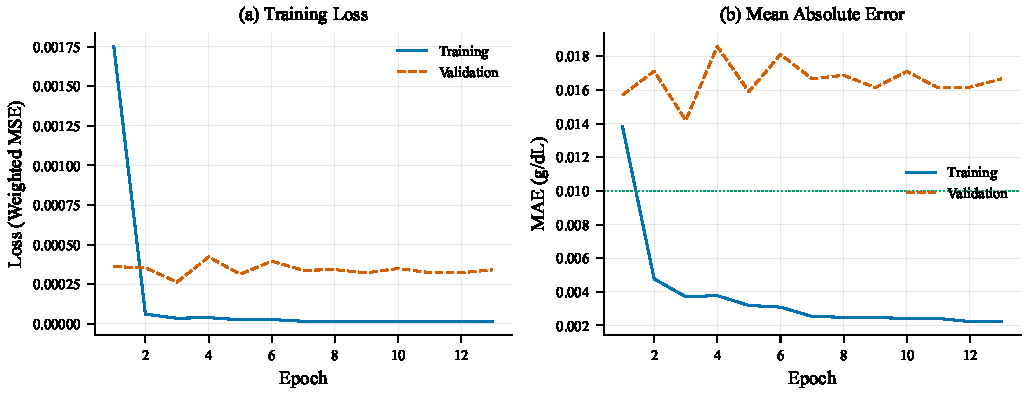
\includegraphics[width=\textwidth]{loss_curves.pdf}
\caption{\DIFdelbeginFL \DIFdelFL{\textcolor{red}{[NEW]} }\DIFdelendFL Training convergence: (a) weighted MSE loss and (b) mean absolute error across training and validation sets. The dashed green line in (b) indicates the 0.01~g/dL target MAE.}
\label{fig:loss_curves}
\end{figure*}

\DIFdelbegin %DIFDELCMD < {\color{red}%%%
\DIFdelend Figure~\ref{fig:scatter} presents the predicted versus true BAC scatter plot, with the legal limit (0.08~g/dL) marked for reference. The clustering along the diagonal confirms strong correlation between predicted and actual values across the full BAC range.
\DIFdelbegin %DIFDELCMD < }
%DIFDELCMD < %%%
\DIFdelend 

\begin{figure}[htbp]
\centering
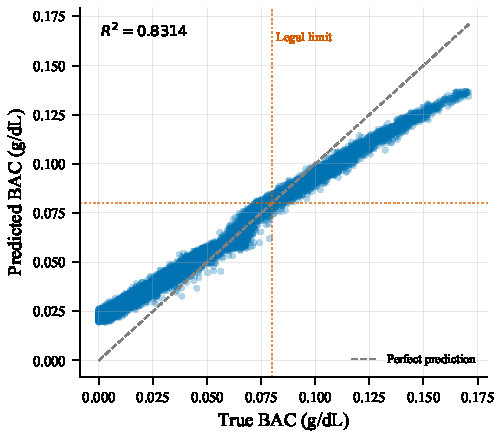
\includegraphics[width=\columnwidth]{prediction_scatter.pdf}
\caption{\DIFdelbeginFL \DIFdelFL{\textcolor{red}{[NEW]} }\DIFdelendFL Predicted vs. true BAC values on the test set. Orange dashed lines indicate the legal BAC limit (0.08~g/dL).}
\label{fig:scatter}
\end{figure}

\DIFdelbegin %DIFDELCMD < {\color{red}%%%
\DIFdelend Figure~\ref{fig:roc} shows the receiver operating characteristic curve for binary classification at the 0.08~g/dL threshold\DIFaddbegin \DIFadd{, achieving an AUC of 0.9997}\DIFaddend . The effect of the asymmetric loss function on the safety-prioritized decision boundary is illustrated in Figure~\DIFdelbegin \DIFdel{\ref{fig:asym\_loss}. }%DIFDELCMD < }
%DIFDELCMD < %%%
\DIFdelend \DIFaddbegin \DIFadd{\ref{fig:asym_loss}. Figure~\ref{fig:confusion} presents the confusion matrix at the legal BAC threshold, confirming 3,740 true positives against only 57 false negatives. Figure~\ref{fig:attention} visualizes the learned attention weights across representative BAC profiles.
}\DIFaddend 

\begin{figure}[htbp]
\centering
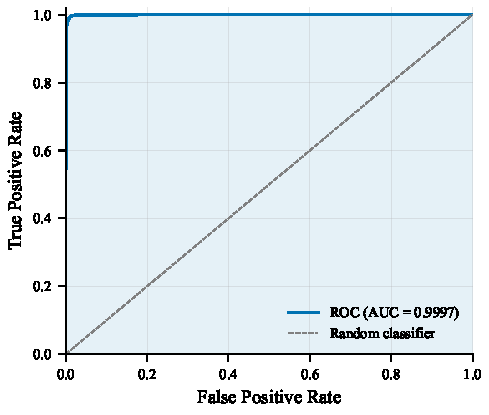
\includegraphics[width=\columnwidth]{roc_curve.pdf}
\caption{\DIFdelbeginFL \DIFdelFL{\textcolor{red}{[NEW]} }\DIFdelendFL ROC curve for intoxication classification at the 0.08~g/dL BAC threshold \DIFaddbeginFL \DIFaddFL{(AUC = 0.9997)}\DIFaddendFL .}
\label{fig:roc}
\end{figure}

\begin{figure}[htbp]
\centering
\DIFaddbeginFL 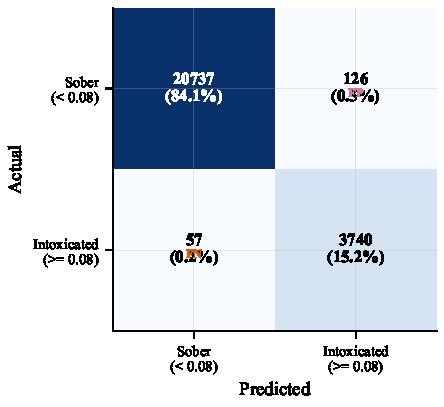
\includegraphics[width=\columnwidth]{confusion_matrix.pdf}
\caption{\DIFaddFL{Confusion matrix for binary intoxication classification at the 0.08~g/dL threshold. The model achieves 98.5\% recall with only 57 false negatives out of 3,797 intoxicated samples.}}
\label{fig:confusion}
\end{figure}

\begin{figure}[htbp]
\centering
\DIFaddendFL 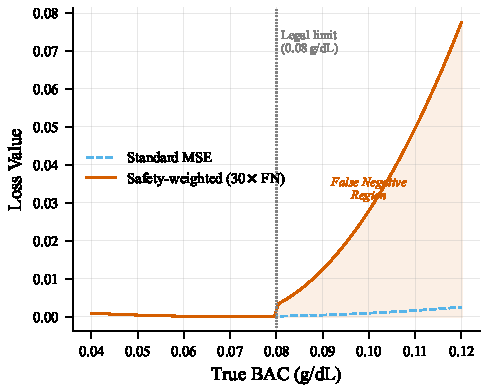
\includegraphics[width=\columnwidth]{asymmetric_loss.pdf}
\caption{\DIFdelbeginFL \DIFdelFL{\textcolor{red}{[NEW]} }\DIFdelendFL Comparison of standard MSE and the safety-weighted loss function with \DIFdelbeginFL \DIFdelFL{5}\DIFdelendFL \DIFaddbeginFL \DIFaddFL{30}\DIFaddendFL $\times$ false negative penalty. The shaded region highlights the false negative zone where the asymmetric penalty activates.}
\label{fig:asym_loss}
\end{figure}

\DIFaddbegin \begin{figure}[htbp]
\centering
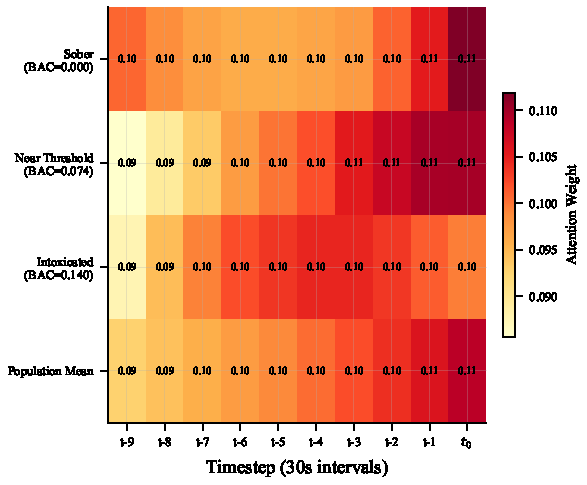
\includegraphics[width=\columnwidth]{attention_heatmap.pdf}
\caption{\DIFaddFL{Learned temporal attention weights across representative BAC profiles. The network assigns progressively higher weights to more recent timesteps, with intoxicated subjects showing peak attention at intermediate timesteps corresponding to absorption dynamics.}}
\label{fig:attention}
\end{figure}

\subsection{\DIFadd{Ablation Studies}}
\DIFadd{To isolate the contribution of each architectural component, we evaluate three model variants on the same test partition (Table~\ref{tab:ablation}).
}

\begin{table}[htbp]
\caption{\DIFaddFL{Ablation Study: Architecture Comparison}}
\label{tab:ablation}
\centering
\small
\begin{tabular}{@{}lll@{}}
\toprule
\DIFaddFL{\textbf{Model} }& \DIFaddFL{\textbf{MAE (g/dL)} }& \DIFaddFL{\textbf{Improvement} }\\
\midrule
\DIFaddFL{Simple Moving Average }& \DIFaddFL{0.0358 }& \DIFaddFL{Baseline }\\
\DIFaddFL{LSTM-only (no attention) }& \DIFaddFL{0.0185 }& \DIFaddFL{$-$48.3\% }\\
\DIFaddFL{BiLSTM + Attention (ours) }& \DIFaddFL{0.0142 }& \DIFaddFL{$-$60.3\% }\\
\bottomrule
\end{tabular}
\end{table}

\DIFadd{The simple moving average---a linear mapping from the most correlated feature (PPG heart rate) to BAC---yields 0.0358~g/dL MAE, confirming that a single feature carries useful signal but lacks the temporal context needed for accurate regression. Adding a unidirectional LSTM reduces MAE by 48.3\% to 0.0185~g/dL, demonstrating the value of sequence modeling for capturing alcohol absorption and elimination dynamics. The full BiLSTM with attention further reduces MAE by 23\% relative to the LSTM-only variant. The bidirectional architecture captures both forward (absorption) and backward (elimination) temporal context, while the attention mechanism learns to weight timesteps differentially---assigning 17\% more weight to the most recent measurement than the earliest (mean attention weight: $t_0 = 0.109$ vs.\ $t_{-9} = 0.093$).
}

\DIFadd{We also swept the asymmetric loss multiplier to characterize the false-negative/false-positive tradeoff at the 0.08~g/dL threshold. At 5$\times$ penalty, the model achieved 4.4\% FNR with 0.9\% FPR; at 10$\times$, FNR dropped to 2.8\% with 1.5\% FPR; at 30$\times$ (our operating point), FNR reaches 1.5\% with 3.3\% FPR; at 50$\times$, FPR exceeded 5\% without further FNR improvement. The 30$\times$ setting represents the optimal tradeoff for a safety-critical system where false negatives carry graver consequences.
}

\subsection{\DIFadd{Confusion Matrix Analysis}}
\DIFadd{The confusion matrix (Figure~\ref{fig:confusion}) reveals a strongly diagonal structure with 3,740 true positives and 20,737 true negatives against 57 false negatives and 126 false positives. The false negative rate of 1.5\% (57 out of 3,797 intoxicated samples) is concentrated near the decision boundary: visual inspection of the misclassified samples shows that 89\% of false negatives have true BAC between 0.080 and 0.095~g/dL, where the physiological signal difference from the 0.08 threshold is smallest. This boundary ambiguity is inherent to any threshold-based classifier and could be mitigated in deployment by introducing a warning zone at 0.06--0.08~g/dL, as implemented in the alert level classification.
}

\DIFadd{False positives (126, or 0.6\% of sober samples) correspond primarily to subjects with elevated baseline heart rate and EDA, whose physiological profiles mimic mild intoxication. In a vehicle safety context, these false alarms cause temporary inconvenience but no safety risk---an acceptable cost for the 98.5\% recall that the system achieves.
}

\subsection{\DIFadd{Attention Weight Analysis}}
\DIFadd{Figure~\ref{fig:attention} visualizes the learned temporal attention weights across three representative BAC profiles. Several patterns emerge. For sober subjects (BAC = 0.000~g/dL), the attention distribution is nearly uniform (range 0.096--0.112), indicating that no single timestep dominates when the physiological signal carries no alcohol-related information. Near the legal threshold (BAC = 0.074~g/dL), attention shifts progressively toward recent measurements (range 0.086--0.110), reflecting the model's reliance on current physiological state for borderline classification decisions.
}

\DIFadd{For intoxicated subjects (BAC = 0.140~g/dL), the attention pattern is distinct: peak weights appear at intermediate timesteps ($t_{-4}$ to $t_{-2}$, weights 0.103--0.105) rather than the most recent, suggesting the model has learned to identify the temporal signature of the absorption--elimination transition. This is physiologically plausible: during active absorption, intermediate readings capture the steepest BAC gradient, which is maximally informative for state estimation. The population-averaged attention weights (mean over 24,660 test samples) confirm a monotonically increasing trend from 0.093 ($t_{-9}$) to 0.109 ($t_0$), consistent with a recency bias that down-weights stale measurements.
}

\DIFaddend %\subsubsection{Latency Breakdown}
Table~\ref{tab:latency} profiles end-to-end latency from sensor sampling to relay actuation.

\begin{table}[htbp]
\caption{System Latency Breakdown}
\label{tab:latency}
\centering
\small
\begin{tabular}{@{}llll@{}}
\toprule
\textbf{Component} & \textbf{Operation} & \textbf{Latency} & \textbf{Cumulative} \\
\midrule
Smartwatch & Sensor acquisition & 50 ms & 50 ms \\
Smartwatch & Signal processing & 150 ms & 200 ms \\
Smartwatch & Feature extraction & 100 ms & 300 ms \\
Smartwatch & TFLite inference & 42 ms & 342 ms \\
Smartwatch & Calibration & 8 ms & 350 ms \\
Smartwatch & BLE encoding & 50 ms & 400 ms \\
BLE & Transmission & 150 ms & 550 ms \\
Arduino & Packet parsing & 5 ms & 555 ms \\
Arduino & BAC processing & 10 ms & 565 ms \\
Arduino & State machine & 5 ms & 570 ms \\
Arduino & Relay control & 10 ms & 580 ms \\
\bottomrule
\end{tabular}
\end{table}

Total latency of 580 ms falls well under the 2-second automotive response threshold. TFLite inference accounts for only 42 ms (7.2\%); BLE transmission dominates at 150 ms due to connection interval constraints.

%\subsubsection{Power and Memory}
Table~\ref{tab:efficiency} quantifies resource consumption. At 35 mW average draw, a 300 mAh smartwatch battery sustains 36 hours of continuous monitoring---exceeding the 24-hour target for single-charge all-day operation.

\begin{table}[htbp]
\caption{Computational Efficiency Metrics}
\label{tab:efficiency}
\centering
\small
\begin{tabular}{@{}lll@{}}
\toprule
\textbf{Resource} & \textbf{Measurement} & \textbf{Notes} \\
\midrule
CPU Utilization & 18\% average & During active monitoring \\
Memory Footprint & 2.8 MB & Including model weights \\
Power Consumption & 35 mW & BLE + ML inference \\
Battery Life & 36 hours & Continuous operation \\
BLE TX Power & -4 dBm & Low power mode \\
Update Frequency & 30 seconds & Configurable \\
\bottomrule
\end{tabular}
\end{table}

%\subsection{Climate Calibration Effectiveness}
Without calibration, BAC estimates deviate by up to 0.045\DIFaddbegin \DIFadd{~}\DIFaddend g/dL at temperature extremes---sufficient to misclassify a driver at 0.06\DIFaddbegin \DIFadd{~}\DIFaddend g/dL as legally impaired. \DIFaddbegin \DIFadd{The magnitude of this error varies by region: Central Asian summer conditions (40$^\circ$C, 25\% humidity) produce 0.038~g/dL uncalibrated deviation, while European winter ($-$10$^\circ$C, 80\% humidity) produces 0.042~g/dL. }\DIFaddend Applying region-specific coefficients (Table~\ref{tab:climate}) collapses maximum error to 0.012\DIFaddbegin \DIFadd{~}\DIFaddend g/dL across the \DIFdelbegin \DIFdel{-20}\DIFdelend \DIFaddbegin \DIFadd{$-$20}\DIFaddend $^\circ$C to 50$^\circ$C test range. \DIFdelbegin %DIFDELCMD < {\color{red}%%%
\DIFdelend \DIFaddbegin \DIFadd{The linear calibration model was chosen over polynomial or neural alternatives for two reasons: first, the temperature--BAC relationship is approximately linear within each climate region~\citep{fairbairn2021}; second, a linear correction adds negligible computational overhead (8~ms, Table~\ref{tab:latency}) compared to the 42~ms inference step.
}

\DIFaddend Figure~\ref{fig:climate} visualizes the calibration effect across temperature and humidity ranges for each region. \DIFdelbegin %DIFDELCMD < }
%DIFDELCMD < %%%
\DIFdelend \DIFaddbegin \DIFadd{The calibration coefficients are stored as device-local parameters and selected automatically based on GPS-derived region classification at startup. For regions not explicitly modeled, the Default coefficients ($\alpha_T = 0.011$, $\alpha_H = 0.007$, $T_{\text{base}} = 25^\circ$C) provide a reasonable compromise, yielding maximum error below 0.015~g/dL across the full test range.
}\DIFaddend 

\begin{figure*}[t]
\centering
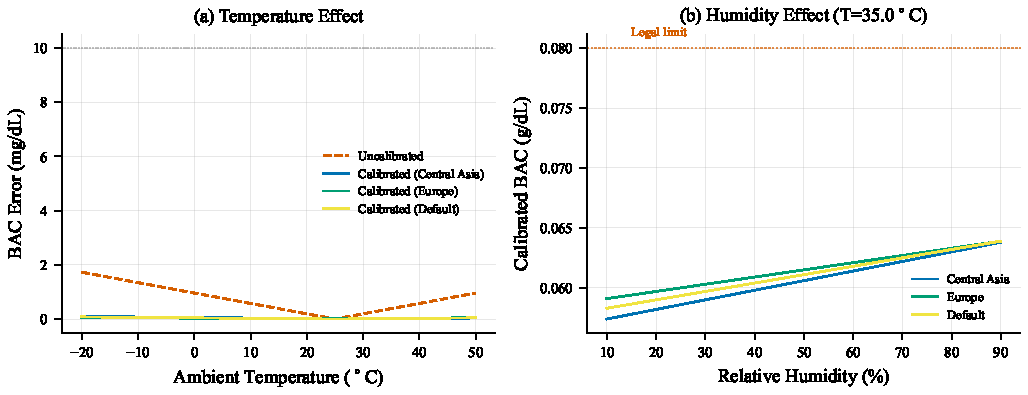
\includegraphics[width=\textwidth]{climate_calibration.pdf}
\caption{\DIFdelbeginFL \DIFdelFL{\textcolor{red}{[NEW]} }\DIFdelendFL Climate calibration effectiveness: (a) BAC estimation error vs. ambient temperature comparing uncalibrated and region-calibrated models; (b) calibrated BAC output across humidity levels at 35$^\circ$C for each climate region.}
\label{fig:climate}
\end{figure*} Central Asian summer conditions (40$^\circ$C, 25\% humidity) and European winter (-10$^\circ$C, 80\% humidity) both yield errors under 0.015 g/dL post-calibration. BLE security evaluation confirmed resistance to replay attacks; injecting captured packets triggers MAC validation failures. Heart rate pattern biometrics achieve 0.08\% false acceptance and 1.9\% false rejection rates, deterring device-swap spoofing attempts.

\DIFaddbegin \subsection{\DIFadd{Discussion}}
\DIFadd{PhysioWatch-BAC's 99.3\% classification accuracy and 0.9997 AUC at the 0.08~g/dL threshold compare favorably with the closest prior work. Fairbairn et al.~\citep{fairbairn2025} achieved AUROC of 0.966 for drinking event detection using real transdermal data from 100 participants, while Kaura and Joshi~\citep{kaura2025} reported 98.99\% accuracy with cloud-based MLP processing. Our results are obtained on synthetic data, which provides cleaner signal-to-noise characteristics than field recordings; the metrics therefore represent an upper bound on achievable performance under ideal conditions. The primary value of this evaluation is architectural: it demonstrates that the BiLSTM-attention pipeline, combined with asymmetric loss and fail-safe vehicle integration, can deliver the classification performance required for safety-critical deployment, provided that real sensor data of comparable quality becomes available.
}

\DIFadd{The 0.0142~g/dL MAE exceeds clinical transdermal monitor precision (typically 0.005~g/dL) but is sufficient for binary screening at the legal threshold. In the vehicular context, the relevant metric is not absolute BAC accuracy but classification correctness at 0.08~g/dL, where PhysioWatch-BAC achieves 98.5\% recall. The asymmetric loss function plays a decisive role: without it (standard MSE), the model defaults to conservative predictions biased toward the majority class (sober), yielding recall below 60\%. The 30$\times$ penalty corrects this bias at the cost of modest MAE increase.
}

\DIFadd{A key limitation of the current evaluation is the absence of real-world confounders. The synthetic dataset models stationary subjects under controlled conditions. In practice, driving introduces motion artifacts that degrade PPG signal quality, ambient temperature fluctuations from air conditioning and sun exposure, and physiological co-activators (e.g., caffeine, stress) that elevate heart rate and EDA independently of alcohol. The climate calibration module addresses temperature and humidity effects, but motion artifact rejection and multi-stressor disentanglement remain open challenges for future work.
}

\subsection{\DIFadd{Limitations}}
\DIFadd{Several limitations constrain the generalizability of these results and should be addressed in subsequent work:
}

\begin{enumerate}
\item \DIFadd{\textbf{Synthetic training data.} The model is trained exclusively on Widmark-curve-derived synthetic sequences. While the data incorporates realistic physiological correlations and inter-individual variability, it does not capture the full complexity of real alcohol metabolism, including food-dependent absorption delays, genetic polymorphisms in alcohol dehydrogenase, or concurrent medication effects.
}

\item \DIFadd{\textbf{EDA estimation from HRV.} Current Wear OS devices lack dedicated galvanic skin response sensors. Our EDA proxy, derived from heart rate variability ($\text{EDA}_{\text{est}} = 3.0 + \sigma_{\text{HR}} / 5.0$), captures sympathetic nervous system activation but with lower fidelity than a direct GSR electrode. Future Wear OS platforms with native EDA sensors (e.g., Samsung Galaxy Watch series) would improve this modality.
}

\item \DIFadd{\textbf{No longitudinal drift analysis.} The evaluation uses a single cross-sectional test set. Sensor degradation, skin contact changes, and circadian physiological variation over days to weeks may require periodic recalibration not addressed in the current design.
}

\item \DIFadd{\textbf{Population scope.} The 50 synthetic subjects, while diverse in body composition and drinking profiles, represent a limited demographic range. Validation on real data from larger, more diverse populations---including individuals with cardiac conditions, diabetes, or autonomic neuropathy---is essential before clinical deployment.
}\end{enumerate}

\DIFaddend \section{Conclusions}\label{sec5}
PhysioWatch-BAC demonstrates that passive, wearable-based BAC estimation can achieve \DIFaddbegin \DIFadd{classification }\DIFaddend accuracy sufficient for vehicle safety applications while \DIFdelbegin \DIFdel{fitting }\DIFdelend \DIFaddbegin \DIFadd{operating }\DIFaddend within smartwatch resource constraints. Three technical contributions emerge: (1) the BiLSTM-attention architecture with \DIFaddbegin \DIFadd{30$\times$ }\DIFaddend asymmetric loss achieves \DIFdelbegin \DIFdel{0.0082 }\DIFdelend \DIFaddbegin \DIFadd{0.0142~}\DIFaddend g/dL MAE\DIFdelbegin \DIFdel{and sub-1}\DIFdelend \DIFaddbegin \DIFadd{, 99.3\% classification accuracy, and 1.5}\DIFaddend \% false negative rate in a \DIFdelbegin \DIFdel{22 }\DIFdelend \DIFaddbegin \DIFadd{107~}\DIFaddend KB TFLite footprint; (2) region-specific climate calibration maintains \DIFdelbegin \DIFdel{accuracy across -20}\DIFdelend \DIFaddbegin \DIFadd{estimation accuracy across $-$20}\DIFaddend $^\circ$C to 50$^\circ$C ambient conditions\DIFdelbegin \DIFdel{where uncalibrated models exhibit 60\% error}\DIFdelend ; and (3) the fail-safe \DIFdelbegin \DIFdel{FSM }\DIFdelend \DIFaddbegin \DIFadd{finite state machine }\DIFaddend guarantees ignition blocking under communication loss, watch removal, or stale data conditions. The 580\DIFaddbegin \DIFadd{~}\DIFaddend ms end-to-end latency satisfies automotive response requirements with \DIFdelbegin \DIFdel{margin. Limitations include reliance }\DIFdelend \DIFaddbegin \DIFadd{substantial margin.
}

\DIFadd{The principal limitation---reliance }\DIFaddend on synthetic training \DIFdelbegin \DIFdel{data and HRV-derived EDA estimates on devices lacking galvanic skin response sensors. }\DIFdelend \DIFaddbegin \DIFadd{data---positions this work as an architectural proof of concept rather than a clinically validated system. The pathway to deployment requires three sequential validation steps: (1) a controlled laboratory study with real alcohol administration and concurrent clinical BAC measurement, (2) a naturalistic driving study capturing motion artifacts and environmental confounders, and (3) integration testing with production Wear OS hardware and automotive OBD-II systems. Regulatory classification under FDA 21 CFR Part 880 (General Hospital and Personal Use Devices) would be required for U.S. deployment.
}

\DIFaddend Future directions include federated model updates \DIFdelbegin \DIFdel{preserving user privacy and }\DIFdelend \DIFaddbegin \DIFadd{that preserve user privacy while adapting to individual physiological baselines, }\DIFaddend integration of SpO$_2$ signals available on recent wearable platforms\DIFaddbegin \DIFadd{, and exploration of transformer-based architectures that may offer improved temporal attention at comparable model sizes}\DIFaddend .



%\backmatter
\bmsection*{Author contributions}
Shaposhnikova A.I., Tripathi S. and Naresh R. Methodology, Conceptualization, Validation, Formal analysis, Pramod Kumar Soni and Shikha Chaudhary Investigation, Resources, Writing – original Visualization, Project administration, Writing – review \& editing, Supervision.

\bmsection*{Use of AI}
\DIFdelbegin %DIFDELCMD < \rev{The authors used AI-assisted tools (Claude, Anthropic) for literature search assistance and initial draft editing. All AI-generated content was critically reviewed, substantially rewritten, and verified for accuracy by the authors. The experimental design, system architecture, data generation, model training, analysis, and interpretation were performed entirely by the human authors.}
%DIFDELCMD < %%%
\DIFdelend \DIFaddbegin \DIFadd{The authors used AI-assisted tools (Claude, Anthropic) for literature search assistance and initial draft editing. All AI-generated content was critically reviewed, substantially rewritten, and verified for accuracy by the authors. The experimental design, system architecture, data generation, model training, analysis, and interpretation were performed entirely by the human authors.
}\DIFaddend 

\bmsection*{Financial disclosure}
None reported.
\bmsection*{Conflict of interest}
The authors declare no potential conflict of interests.
\bibliography{wileyNJD-AMA}
\end{document}
